
%
% Einfache LaTeX-Vorlage f�r Arbeiten am Lehrstuhl Kranzlm�ller / MNM-Team
% - optimiert f�r die Arbeit mit g�ngigen LaTeX-Editoren
% - funktioniert ohne Makefile und Anpassungen der LaTeX-Verzeichnisstruktur
% - verwendet Komaskript f�r ein (nach europ�ischen Gepflogenheiten) sch�neres Layout
% 
% v1, 2007 (Michael Brenner)
% Diese Version: v1.1, 2012 (Michael Brenner)
%


\documentclass[bibliography=totoc,listof=totoc,BCOR=5mm,DIV=12]{scrbook} % Rand f�r Bindung: 5mm / falls Index verwendet, erg�nze "index=totoc" zu den Optionen 
% \usepackage{bibgerm}       % deutsche Literaturverzeichnisse
\usepackage{courier}
\usepackage[dvipsnames]{xcolor}
\usepackage{gensymb}
\usepackage[inline]{enumitem}
\usepackage[latin1]{inputenc} % Umlaute im Text
\usepackage{listings}
\usepackage{pdfpages}
\usepackage{attachfile2}
\addtokomafont{labelinglabel}{\sffamily}

\newcommand\realnumberstyle[1]{}

\makeatletter
\newcommand{\zebra}[3]{%
    {\realnumberstyle{#3}}%
    \begingroup
    \lst@basicstyle
    \ifodd\value{lstnumber}%
        \color{#1}%
    \else
        \color{#2}%
    \fi
        \rlap{\hspace*{\lst@numbersep}%
        \color@block{\linewidth}{\ht\strutbox}{\dp\strutbox}%
        }%
    \endgroup
}
\makeatother

\setcounter{tocdepth}{4}
\setcounter{secnumdepth}{4}

\renewcommand{\topfraction}{0.9}
\renewcommand{\bottomfraction}{0.9}

\lstset { %
    language=C++,
    %backgroundcolor=\color{Black!5}, % set backgroundcolor
    basicstyle=\footnotesize,% basic font setting,
    commentstyle=\color{ForestGreen},
    basicstyle=\footnotesize\ttfamily,
    % breaklines=true,
	numberstyle=\zebra{black!5}{white},
    % numbers=left,
    % firstnumber=1,
    % numberfirstline=true,
    % stepnumber=1,
    keywordstyle=\color{MidnightBlue}
}

\usepackage{graphicx} % Einf�gen von Grafiken  - f�r PDF-Latex: .pdf und .png (.jpg m�glich, sollte aber vermieden werden)
\usepackage{mathtools}		% sch�nere Summenzeichen usw
\usepackage{mathrsfs}		% kursive Buchstaben
\usepackage{url}           % URL's (z.B. in Literatur) sch�ner formatieren
\usepackage{hyperref} % sorgt f�r f�r Hyperlinks in PDF-Dokumenten
%\usepackage{cite}
\usepackage[noadjust]{cite}
\graphicspath{{./Bilder/}}
\usepackage[section]{placeins}

%
% der Befehl \hypenation versteht keine Sonderzeichen, also weder �
% noch "a noch \"a. W�rter die derartige Zeichen enthalten m�ssen
% direkt im Text getrennt werden, z.B. W�r\-ter
%
\hyphenation{Ma-nage-ment}
\hyphenation{Ma-nage-ment-agent}
\hyphenation{Ma-nage-ment-agent-en}
\hyphenation{Ma-nage-ment-ar-chi-tek-tur}
\hyphenation{Ma-nage-ment-ar-chi-tek-tu-ren}
\hyphenation{Ma-nage-ment-an-wen-dung}
\hyphenation{Ma-nage-ment-an-wen-dung-en}
\hyphenation{Ma-nage-ment-an-for-der-ung}
\hyphenation{Ma-nage-ment-funk-ti-on}
\hyphenation{Ma-nage-ment-funk-ti-onen}
\hyphenation{Ma-nage-ment-kon-zep-te}
\hyphenation{Ma-nage-ment-res-source}
\hyphenation{Ma-nage-ment-in-for-ma-ti-on}
\hyphenation{Ma-nage-ment-res-sour-cen}
\hyphenation{ma-nage-ment-re-le-vante}
\hyphenation{ma-nage-ment-sy-stem}
\hyphenation{ma-nage-ment-sy-steme}
\hyphenation{Ma-nage-ment-in-stru-men-tie-rung}
\hyphenation{Ma-nage-ment-platt-form}
\hyphenation{Sys-te-men}
\hyphenation{Sys-tem-um-ge-bun-gen}
\hyphenation{Sys-tem-ma-nage-ment}
\hyphenation{DHCP}
\hyphenation{Ma-nage-ment-diszi-plinen}
\hyphenation{System-management-architekturen}
\hyphenation{Verwendungs-nachweise}
\hyphenation{Video-einricht-ungen}
\hyphenation{Res-source}
\hyphenation{Res-sourcen}
\hyphenation{Grund-anwendung}
\hyphenation{Grund-anwendungen}
\hyphenation{Basis-anwendung}
\hyphenation{Core}
\hyphenation{Kom-mu-ni-ka-ti-on}
\hyphenation{De-sign-ent-schei-dung}
\hyphenation{Sprung-ad-res-sen}
\hyphenation{Klas-si-fi-ka-ti-on}
\hyphenation{Schreib-recht}
\hyphenation{Be-nut-zer-zer-ti-fi-kat}
\hyphenation{Bau-stein-ent-wi-ckler}
\hyphenation{ad-mi-ni-stra-ti-ve}

 % in dieses File kommen W�rter die Latex nicht richtig trennt

\begin{document}

% ---------------------------------------------------------------
\frontmatter % Titelbl�tter und Erkl�rung jeweils spezifisch f�r die jeweilige Uni einbinden
    %%%%%%%%%%%%%%%%%%%%%%%%%%%%%%%
% erste Seite

\thispagestyle{empty}

\begin{center}

\vspace*{-2cm}

{\Huge INSTITUT F�R INFORMATIK\\[1mm]}
DER LUDWIG--MAXIMILIANS--UNIVERSIT�T M�NCHEN\\

\vspace*{1cm}


\includegraphics[width=0.3\textwidth]{lmu_siegel}

\vspace*{2cm}

{\Large \textbf{Master's Thesis}}\\ % oder Fortgeschrittenenpraktikum, Master's Thesis, Bachelorarbeit etc.

\vspace{2.0cm}
{\Huge \textbf{Evaluation of Virtual Reality based Mesh Saliency Maps}}\\
% \vspace*{3mm}
% {\Huge \textbf{-- additional line}}\\
\vspace{1.5cm}

{\LARGE Richard Metzler} % Name des Autors

\vspace{3cm}
Draft vom \today % erleichtert den Betreuern die Zuordnung - f�r finale Version entfernen

\end{center}

\newpage

%%%%%%%%%%%%%%%%%%%%%%%%%%%%%%%
% zweite Seite

\thispagestyle{empty}
\cleardoublepage

%%%%%%%%%%%%%%%%%%%%%%%%%%%%%%%
% dritte Seite (Kopie der ersten)

\thispagestyle{empty}

\begin{center}

\vspace*{-2cm}

{\Huge INSTITUT F�R INFORMATIK\\[1mm]}
DER LUDWIG--MAXIMILIANS--UNIVERSIT�T M�NCHEN\\

\vspace*{1cm}


\includegraphics[width=0.3\textwidth]{lmu_siegel}

\vspace*{2cm}

{\Large \textbf{Master's Thesis}}\\ % oder Fortgeschrittenenpraktikum, SEP etc.

\vspace{2.0cm}
{\Huge \textbf{Evaluation of Virtual Reality based Mesh Saliency Maps}}\\
% \vspace*{3mm}
% {\Huge \textbf{-- additional line}}\\
\vspace{1.5cm}

\vspace{1.5cm}

{\LARGE Richard Metzler} % Name des Autors
\vspace{2cm}

\parbox{1cm}{
\begin{large}
\begin{tabbing}
Aufgabensteller: \hspace{.5cm} \=Prof. Dr. Dieter Kranzlm�ller\\[2mm]
Betreuer:
\>Markus Wiedemann\\ % alphabetische Reihenfolge (Nachname)
%\>MNM-Team-Betreuer 2\\
%\>Externer Betreuer 1 (Firma)\\[5mm]
Abgabetermin: \> 29. September 2017\\
\end{tabbing}
\end{large}}\\
\vspace{5mm}

\end{center}
 % Titelbl�tter LMU - auskommentieren falls TUM-Arbeit
%    % Richtlinien, siehe http://wwwpa.in.tum.de/generell/Abschlussarbeitsform.html
%
%%%%%%%%%%%%%%%%%%%%%%%%%%%%%%%


% Deckblatt

\thispagestyle{empty}

\begin{center}
    
\includegraphics[width=3cm]{tum-logo}\\
    \vspace{.5cm}
% "Technische Universit�t M�nchen" oder alternativ das Logo der TUM
    {\Large \sc Technische Universit�t M�nchen}\\

    \vspace{1cm}
% "Fakult�t f�r Informatik"
    {\Huge \sc Fakult�t f�r Informatik\\[1mm]}


    \vspace{2cm}
% Diplomarbeit | Master's Thesis | Bachelorarbeit in Informatik | Wirtschaftsinformatik |
    {\Large \textbf{Diplomarbeit in Informatik}}\\
% Thema bzw. Titel der Arbeit  (In der Sprache, in der die Arbeit verfasst wurde)
    \vspace{2.0cm}
    {\Huge \textbf{Ein Lorem-Rahmenwerk}}\\ % bei langen Titeln ggf. Schriftgr��e auf \huge herunter setzen
    \vspace*{3mm}
    {\Huge \textbf{f�r Ipsum-Systeme}}\\
    \vspace*{3mm}
    {\Huge \textbf{-- ein Dolor-Ansatz}}\\
    \vspace{1.5cm}
% Vorname und Nachname des Bearbeiters/ der Bearbeiterin
    Vorname Nachname

    \vspace{5cm} % ggf. je nach Zeilenzahl und Schriftgr��e des Titels anpassen
    
\includegraphics[width=2.4cm]{tum-info-logo}
\end{center}

\newpage

%%%%%%%%%%%%%%%%%%%%%%%%%%%%%%%
% R�ckseite Deckblatt

\thispagestyle{empty}
\cleardoublepage

%%%%%%%%%%%%%%%%%%%%%%%%%%%%%%%
% Erste Seite (Titelblatt)

\thispagestyle{empty}

\begin{center}

    
\includegraphics[width=3cm]{tum-logo}\\
    \vspace{.5cm}
    {\Large \sc Technische Universit�t M�nchen}\\


    \vspace{.5cm}

    {\huge \sc Fakult�t f�r Informatik\\[1mm]}


    \vspace{1cm}

    {\Large \textbf{Diplomarbeit in Informatik}}\\ % oder SEP etc.

% Thema bzw. Titel der Arbeit  (In der Sprache, in der die Arbeit verfasst wurde)
    \vspace{1.5cm}
    {\huge \textbf{Ein Lorem-Rahmenwerk}}\\ % bei langen Titeln ggf. Schriftgr��e herunter setzen
    \vspace*{3mm}
    {\huge \textbf{f�r Ipsum-Systeme}}\\
    \vspace*{3mm}
    {\huge \textbf{-- ein Dolor-Ansatz}}\\

% die englische bzw. deutsche Entsprechung des Titels
    \vspace{1cm}
    {\huge \textbf{A Lorem Framework}}\\ % bei langen Titeln ggf. Schriftgr��e herunter setzen
    \vspace*{3mm}
    {\huge \textbf{for Ipsum Systems}}\\
    \vspace*{3mm}
    {\huge \textbf{-- a Dolor Approach}}\\
    \vspace{1cm}

    \parbox{1cm}{
      \begin{large}
        \begin{tabbing}
          Bearbeiter: \hspace{1.5cm}
            \=Vorname Nachname\\[2mm]
    Aufgabensteller: \>Prof. Dr. Dieter Kranzlm�ller\\[2mm]
    Betreuer: \>MNM-Team-Betreuer 1\\ % alphabetische Reihenfolge (Nachname)
    \>MNM-Team-Betreuer 2\\
    \>Externer Betreuer 1 (Firma)\\[5mm]
    Abgabedatum: \> 7. Juli 2077\\
        \end{tabbing}
      \end{large}
    }\\

    \vspace{.3cm}

    
\includegraphics[width=2.4cm]{tum-info-logo}

\end{center}
 % Titelbl�tter TUM - auskommentiert lassen falls LMU-Arbeit
    \thispagestyle{empty}
    \cleardoublepage
    %
% LaTeX-Rahmen f�r Arbeiten am Lehrstuhl Hegering
%
% Harald Roelle, 2001, 2002
%
% basierend auf Arbeiten von Helmut Reiser, Boris Gruschke und Stephen Heilbronner
%

\newpage

\thispagestyle{empty}

\begin{large}

\vspace*{2cm}

\noindent
Hiermit versichere ich, dass ich die vorliegende Masterarbeit
selbst�ndig verfasst und keine anderen als die angegebenen Quellen
und Hilfsmittel verwendet habe.

\vspace{2cm}

\noindent
M�nchen, den 29. September 2017

\vspace{3cm}

\hspace*{7cm}%
\dotfill\\
\hspace*{8.5cm}%
\textit{(Unterschrift des Kandidaten)}

\end{large}
 % Erkl�rung (Arbeit selbstst�ndig verfasst) - auskommentieren falls TUM-Arbeit
%    \begin{large}

\vspace*{2cm}
\noindent
Ich versichere, dass ich diese Diplomarbeit % (bzw. Master's Thesis)
selbst�ndig verfasst und nur die angegebenen Quellen und Hilfsmittel verwendet habe.

\vspace{2cm}

\noindent
M�nchen, den 7. Juli 2077

\vspace{3cm}

\hspace*{7cm}%
\dotfill\\
\hspace*{8.5cm}%
\textit{(Unterschrift des Kandidaten)}

\end{large}
 % Erkl�rung (Arbeit selbstst�ndig verfasst) - auskommentiert lassen falls LMU-Arbeit
    \thispagestyle{empty}
    \cleardoublepage
    \begin{center}
    \textbf{Kurzzusammenfassung}
\end{center}

\noindent Im Rahmen dieser Arbeit wird untersucht, welche Teile von 3D Objekten als visuell interessanter empfunden werden als andere und wie sich die \textit{wahrgenommene Wichtigkeit} auf der Oberfl\"ache solcher Modelle verteilt. Zwei grunds\"atzlich verschiedene L\"osungsans�tze zu dieser Frage werden zu Hilfe gezogen. Es werden automatisch, anhand eines mathematisch begr\"undeten Prozesses errechnete Verteilungen von Wichtigkeit betrachtet. Mit diesen Ergebnissen werden Verteilungen wahrgenommener Wichtigkeit verglichen, welche durch direkte Nutzer-Interaktion mit einer Auswahl-Applikation entstanden sind, die im Rahmen dieser Arbeit erstellt wurde. Das Ziel dieser Arbeit ist das Bereitstellen einer Grundlage von Daten, welche den Anfang einer Evaluation von Unterschieden dieser beiden Vorgehensweisen erm\"oglicht.

32 Nutzer nahmen bei der Studie teil, welche durchgef\"uhrt wurde um die Grundlage f\"ur diese Diskussion zu schaffen. Die Teilnehmer nutzten die im Rahmen dieser Arbeit erstellte Software um Punkt-weise Teile von 3D Objekten, die sie als interessant empfanden, zu markieren. Gleichzeitig wurde ein grundlegendes Differenz-Ma{\ss} entwickelt, welches etwaige Unterschiede beschreiben soll. Dieses hat zum Ziel, eine Prozentzahl als Ergebnis zu liefern, welche beschreibt wie stark die durchschnittliche Nutzer-Auswahl von den vorab errechneten Ergebnissen abweicht.

W�hrend eindeutige \"Ahnlichkeiten erkennbar sind und diese sich auch in den Kennzahlen widerspiegeln, besteht diese Evaluation mehr auf qualitative Beschreibungen von Tendenzen und Mustern, da eine fundierte, umfassende Analyse von Unterschieden solcher Datentypen den Rahmen dieser Arbeit gesprengt h\"atte.

\vspace*{1.5cm}

\begin{center}
    \textbf{Abstract}
\end{center}

\noindent The subject of this work is to inspect which parts of 3D objects are visually interesting, which are not, and how \textit{perceived importance} is distributed on the surface of such models. Two fundamentally different approaches to this question are compared in this work. First, \textit{importance maps} computed by an automated, mathematically founded procedure are considered. Second, distributions of perceived importance, based on direct user input, gathered from an application based on virtual reality technology, are considered. The goal of this work is to collect enough data to start an evaluation of differences between the results of these two approaches.

In order to establish a foundation of this discussion, a user study was conducted with 32 participants. They would each use the software developed in the scope of this work to select parts of objects they deemed \textit{interesting}. Beforehand, a basic measure of difference was conceptualised in order to describe differences that were speculated to be found. The goal was to compute one percentage-ratio which, based on vertex-wise comparison of importance values provided by user input and computation, indicates how much the user selection differs from the results of computation.

While there are clear similarities, this evaluation os more based on observation of tendencies and patterns since a sound, exhaustive analysis of differences in such types of data would have gone beyond the scope of this work.

\newpage
 % Abstract
    \thispagestyle{empty}
    \tableofcontents % Inhaltsverzeichnis

% ---------------------------------------------------------------
\mainmatter % die eigentliche Arbeit

	\chapter{Introduction}
\label{sec:introduction}

Beginning in the 1950's, virtual reality technology \cite{steuer1992defining} has been continuously researched and improved and its professional relevance is becoming ever more present today. There is a plentitude of recent works showing that it bears great potential and positive possible contributions to architecture and construction \cite{sampaio2014application}, \cite{le2015social}, \cite{stouffs2013happening}, healthcare and psychotherapy \cite{baus2014moving}, \cite{merians2014rehabilitation}, \cite{de2014healthcare}, engineering and industrial design \cite{marks2014towards}, \cite{wendrich2016hybrid}, gaming and home entertainment \cite{valente2016live}, \cite{zyda2005visual} and education \cite{merchant2014effectiveness}, \cite{ott2015literature}. One must also consider that this technology can help gaining new insights and open up new perspectives into greater, more abstract matters of social, environmental and economic manner \cite{ovtcharova2015innovation}, \cite{nguyen2016applying}. 

With resources such as memory and computing power becoming more and more available at ever-increasing rates, 3D objects and their mesh representations are constantly growing in complexity and size, in terms of shaders, texture maps as well as the sheer number of vertices. Still, many professional applications revolving around interaction with such models require means of displaying them in real-time without significant perceived loss of quality to ensure a smooth and fast workflow. This is where mesh simplification and segmentation plays an important role \cite{wei2010feature}, \cite{shaffer2001efficient}, \cite{zhao2012saliency} etc.

This issue becomes even more pressing in a professional, commercial context where access to state of the art, high-performance graphic processing units or render farms is not a given for everybody. With less computing power available, means of user-oriented, real-time rendering are of vital importance to a fast and unimpeded way of working on 3D assets.

Little has been done so far concerning research on \textit{mesh saliency} on a vertex level in a virtual reality environment. Whether saliency maps computed via known methods affect user behavior immersed in VR scenes at all, or to which extent has not been investigated in a vertex selection scenario. Furthermore, as of now, the effect on perceived visual quality of saliency-based object simplification as well as user behavior when given the opportunity to declare salient regions themselves is barely touched on at all.

For the selection of parts of objects which seem important to beholders, I was able to use the Virtual Reality and Visualisation Centres five-sided projection installation at the Leibniz Supercomputing Centre in Munich. This installation creates interactive, immersive virtual reality environments via multiple projectors and tracking sensors. Users only need to wear a lightweight pair of stereo shutter glasses that are synchronized with the projectors and thus can seperate two images for the spectator - one for each eye. The glasses are equipped with an electromagnetic tracking system so that their exact position, orientation and tilt can be captured in real-time, allowing the computation of the users perspective in 3D scene at any time. Based on this perspective, the projectors use the walls as projection surfaces and throw live images resembling what the user would see if he/she were physically in the virtual scene onto the walls. The projection installation grants a virtual reality experience which is enhanced by the fact that the user only needs to wear a pair of glasses instead of a fully sized headset. From a user perspective, another advantage of such a setup is the fact that there are no cables connected to the glasses which can evoke a feeling of inhibition or the constant worry of stumbling over or accidentally damaging the cables.

% Überleitung hier: Was passiert generell?
% im Absatz oben checken ob eletromagnetic trackers stimmt

Finally, it is worth noting that the effect on perceived quality of objects in 3D scenes that can possibly achieved through saliency-based simplification is not limited to virtual reality applications. Long-term goals of efficiency and optimization will continue to be accompanied by the need for semi-automatic complexity reduction of objects without a great loss of visual appeal, regardless of the type of media they will be presented on. So the best case outcome of this work is to find possible approaches to identifying segments of objects which are of high importance to the average beholder based on the immersive nature of the selection process of said segments.

% Kapitel der Arbeit beschreiben

	\chapter{Related work}
\label{sec:related_work}

This section is subdivided into two parts. First, publications discussing \textit{mesh saliency}, a technique used term to predict regional percieved importance of digital representations of real-world (or synthetic) objects as well as 2D images, will be presented and briefly described. The second section will provide a look into human behavior, based on cognition and outside stimuli in virtual reality environments. These two sets of scientific works will provide a solid knowledge of terms and methods commonly used in this field and describe the current state of the art.

\section{Mesh saliency and human perception}
\label{sec:mesh_saliency_and_human_perception}

Research on what human perception guides us to focus our attention on when presented with an 3D representation of an object was begun just past the year 2000 and has been a continuous effort ever since. One commonly cited publication in this field is Lee \textit{et al.} \cite{lee2005mesh}. Based on low-level human visual attention \cite{koch1987shifts}, it introduces the term \textit{mesh saliency}, a measure for regional based importance of 3D meshes, and also presents a way to compute it. This fully automatic process successfully predicts  what would be classified by most observers as prominent, visually interesting regions on a mesh, thus allowing mesh operations such as simplification \cite{cignoni1998comparison} and segmentation \cite{shamir2008survey} to produce results that are more appealing to the beholder.

\begin{figure}[htb]
  \centering
  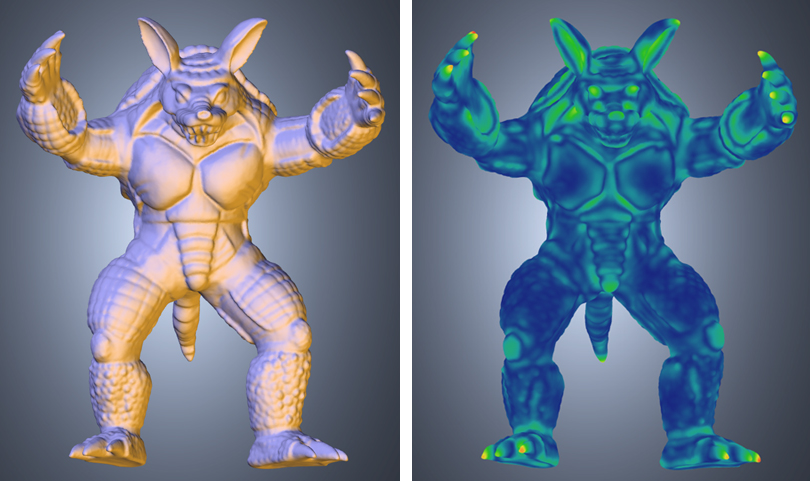
\includegraphics[width=1.0\textwidth]{arma.png}\\ % PNG-File
  \caption{A model and its computes mesh saliency map. Published by Lee \textit{et al.} \cite{lee2005mesh}. Bright colors (yellow and red) indicate high saliency values for their respective vertices, dark colors (shades of blue) indicate low values.}\label{fig:lee_arma_map}
\end{figure}

The model for computing \textit{mesh saliency} is based on a center-surround comparison of local curvature. It is scale-dependent on a \textit{saliency factor} $\varepsilon$, which is based on the diagonal of the objects bounding box, and is able to identify salient features of a mesh, depending on their surrounding area. Geometrically complex regions, for example a large patch containing lots of bumps of similar size, will be rightfully dismissed as, in most cases, regions that are not interesting from a human perceptional stance.

Taking a closer look at the basic formula through which saliency for any vertex of a mesh can be computed according to Lee \textit{et al.} helps understanding the underlying concept. As a first step, the mean curvature map for a mesh, describing mean local curvature values on a point-level for each of its vertices, needs to be calculated via commonly known approaches such as \cite{taubin1995estimating}. The resulting mean curvature map $\mathscr{C}$ defines a mapping from each vertex of a mesh to its mean curvature $\mathscr{C}$(\textit{v}). Using a distance measure such as the Euclidean or geodesic method, one can compute the neighbourhood \textit{N}(\textit{v},$\sigma$) of a vertex \textit{v} which then defines a set of points within a distance $\sigma$. The Euclidean appraoch was used in Lee \textit{et al.} and subsequently in the formula below.
Using these definitions, the authors denote the Gaussian-weighted average of the mean curvature by G($\mathscr{C}$(\textit{v}),$\sigma$) and present the following way of computing it.

\begin{align*}
G(\mathscr{C}(v),\sigma) &= \frac
	{
		\sum_{x \in N(v,2\sigma)}
			\mathscr{C}(x)exp	-||x-v||^2 \backslash(2\sigma^2)
	}{
		\sum_{x \in N(v,2\sigma)}
			exp -||x-v||^2 \backslash(2\sigma^2)
	}
\end{align*}

For computation of the Gaussian-weighted average, a cut-off factor for the filter is assumed at a distance of 2$\sigma$, in other words twice the distance that a vertex can have to another vertex to still be considered in its neighbourhood.
Based on these definitions, the saliency $\mathscr{S}$(\textit{v}) of a vertex \textit{v} is defined as the abslute difference between the Gaussian-weighted averages, as seen in the formula below.

\begin{align*}
\mathscr{S}(\textit{v}) &= |\textit{G}(\mathscr{C}(\textit{v}),\sigma) - G(\mathscr{C}(\textit{v}),2\sigma)|
\end{align*}

In order to get more refined results, one can conduct multiple computations of \textit{mesh saliency} with different values for $\sigma$. Lee \textit{et al.} use the previously mentioned \textit{saliency factor} $\varepsilon$ with $\varepsilon \in [2,6]$ in their paper, to generate multiple values for $\sigma$.

The concept of \textit{mesh saliency} has since been refined, augmented and adapted to serve as a basis for a multitude of specific use-cases and applications. When processing single vertex saliency, Wu \textit{et al.} \cite{wu2013mesh} took into consideration not only the curvature of the region surrounding the vertex, but also the global context of it. In other words, for each vertex to be attributed a value describing its saliency, its \textit{global rarity}, derived from comparing its features to those of every other vertex of the object, is computed. They performed a user study in which they had participants choose one out of two saliency maps for a set of objects, presented in a random order. One map was generated using their approach, the other one with the model presented in Lee \textit{et al.} Participants were asked to pick the one that was a closer representation of what they would have considered interesting regions and features. Since their method got picked in almost 58 per cent of cases, while the results produced by the model presented in Lee \textit{et al.} were favored in about 42 per cent, this can be considered a true improvement of the way \textit{mesh saliency} can be computed.

One approach to improve the method of finding salient elements in 2D images relied on paying extra attention to depth-information in \cite{ciptadi2013depth}. In this work, Ciptadi \textit{et al.} found that better results in terms of automatic identification of objects and surfaces could indeed be achieved this way. Transferring these insights into a 3D context is easy since visually complex models often base on multiple image-maps describing, among other information, depth values on the surfaces of the model.
In \cite{potapova2011learning}, the authors took a more task-driven approach to contribute to the concept of \textit{saliency}. Gathering colour- and depth information about real-world scenes using a Kinect sensor, they extracted semantic cues about surface heights, relative surface orientations and occluded edges. Based on that data, they computed combined saliency maps which allowed them to assign real-world objects to four different categories, enhancing ways a robotic system can interact with them, providing the best possible points where the objects can be grasped and whether they are in reach at all or not (due to occlusion by other objects).

Another recent work aimed at identifying single, distinct elements and objects of 3D models was presented in \cite{koschan2003perception} by Koschan \textit{et al.} The authors propose a segmentation algorithm that utilises a human perception phenomenon known as the \textit{minima rule} which suggests that contours of negative curvature minima can serve as boundaries of disjunct visual parts or elements. Another detailed comparison between automatically detected points of interests and what participants in a study actually declared as visually interesting points was drawn by Dutagaci \textit{et al.} in \cite{dutagaci2012evaluation}.

To verify the practical relevance of identifying salient regions and features on 3D meshes, Howlett \textit{et al.} \cite{howlett2005predicting} conducted a user study on whether it is possible to determine such features in advance. Based on observations gathered from eye-tracking device based user studies, they concluded that, especially with natural objects (animals, humans etc.), this was indeed the case. On top of that, they also reported a significant increase in visual fidelity on objects which were simplified based on saliency weight-maps, according to reports of study participants. Furthermore, in \cite{kho2003user} the authors used user-guided simplification to preserve higher levels of detail in areas of 3D objects that people deemed important to the recognisability of the object. After performing mesh simplification according to \cite{garland1997qslim}, enhanced by taking user-derived weight maps into account, the authors observed what they described as perceptually improved approximations of input objects.

In another highly noteworthy work by Munaretti \cite{munaretti2007perceptual}, the concept of \textit{mesh saliency} was extended to deformable, i.e. animated objects. The author presented a way to generate so-called \textit{multi-pose saliency}, a combination of multiple saliency maps compoted for static poses of a mesh. These static meshes can also be interpreted as keyframed poses for dynamic deformation, which makes this work a potentially outstanding contribution to any field where 3D objects are being animated.

The author found a remarkable improvement of the original way of computing \textit{mesh saliency} as presented by Lee \textit{et al.} by using geodesic distance \cite{surazhsky2005fast} instead of euclidean distance when comparing local curvature values and implemented a way to compute multiple saliency maps for different levels of detail.

\section{Human attention in Virtual Reality}
\label{sec:human_attention_in_virtual_reality}

While navigation in virtual reality space via a traditional desktop setup with input devices such as a mouse and a keyboard still seems to allow users to perform better in basic tasks such as navigation, they generally perceived interaction via a head-mounted display more natural and intuitive \cite{santos2009head}. It is worth noting though, that this work evaluated a series of user studies described in their respective papers which were published between 1997 and 2006. Thus, it is safe to assume that recent VR technology would get much better results in comparison. This was hinted at in the paper multiple times, mentioning the idiosyncrasies of the equipment used in the studies.
The main tasks in the studies described in this paper included navigation (both in small and large-scale virtual environments), searching for certain objects, physically replicating simple virtual sculptures as well as generic volume visualisation tasks (identification, judgement of size, shape and connectivity). Regarding navigation, the authors concluded that during the six considered studies, slightly faster or equal completion times between VR and desktop setup users could be observed. Results for search tasks were found to be more varied. One study reportedly concluded that desktop users were faster, another one stated the opposite. Visualisation tasks such as size estimations were fulfilled with better results by users in a fully immersive virtual environment compared to participants using a head mounted VR display \cite{qi2006comparison}. This is an interesting find for this work since this user study was conducted with the help of so-called fish tank VR \cite{ware1993fish}. This setup, due to the lightweight stereoscopic glasses and almost unrestricted freedom of movement, resembles a very basic variation of the kind of immersive experience that can be achieved with the use of a multi-wall projection installation which I had access to for this work.

Another, in the context of this work, very relevant study described in the paper above is \cite{mizell2002comparing}. This work, aiming at finding measurable advantages of immersive virtual reality (IVR) over conventional display methods within the context of complex 3D geometry, had users cloesly observe sculptures consisting of more or less randomly bent rods of equal thickness. The users - grouped into IVR and desktop users - were asked to physically replicate the fairly complex object with real, easily deformable leaden rods while looking at the virtual object. The paper describes two studies, in one of wich the IVR setup was a multi-sided projection installation, allowing the users to view the geometric data from effectively every possible position and angle while the desktop user group had to use a joystick or control pad for navigation. It reports that IVR users performed consistently superior regarding both time and error-rate. This suggests that immersive virtual technology might be able to offer a more precise understanding of complex geometric data which is a compelling assumption regarding this work.

With the ambition to develop a predictive model for the positive outcome using a VR setup can have compared to its expenses, Pausch \textit{et al.} \cite{pausch1997quantifying} found that, while not being being able to help users perform search tasks in virtual space faster than with a desktop setup, users with a head-mounted display were able to complete the tasks with more certainty. They spent significantly less time re-examining areas, which they commonly did with the desktop setup - up to 41\% more time. The task users were given in this work was to find a specific letter hidden on the walls of a virtual room which were textured with evenly spread sets of letters, or confidently declare that the letter wasn't present. The target letter was not actually present in the room in 50\% of the tests. Based on the observation that VR users in this study barely spent any time rescanning parts of the virtual room, the authors assumed that a VR setup can have a greatly beneficial impact on systematic search tasks. They based this on the fact that spatial understanding and navigation skills are naturally very well developed parts of human cognition and proposed that the immersive experience did such a sufficiently well job at mimicking a real life environment that these skills could be used to a greater extent than in a desktop setup. Again, this is further reason to be optimistic about finding interesting patterns in what users in a VR setup find to be highly significant regions of 3D objects.

Taking a step back towards the basics of human attention in 3D space, in 1998, Atchley \textit{et al.} \cite{atchleyattentional} conducted four experiments addressing attention in 3D scenes on a very basic level. Participants were shown simple scenes, each containing sets of six short lines. The scenes were arranged on four different depth planes, one behind the other, and displayed on a stereographic display. The basic task given to participants in all of the experiments was to focus a briefly visible colour singleton on a specific, previously cued depth plane. One of the lines on the indicated plane would change its colour for 100 milliseconds and participants had to correctly say whether it was tilted to the left or the right. To determine the time it takes to shift attention from one plane to another, for some user groups, the colour singleton would appear in a plane other than the previously hinted one. To further track speed and accuracy of attention focus, a distraction element (one additional line changing its colour simultaneously to the target line) was shown to some participants, sometimes in the \textit{target plane}, sometimes in a different one. From their observations, the authors gathered that depth-plane attention can be successfully guided and that distraction elements appearing on the \textit{target plane} significantly interfered with the users' ability to give correct answers, while such elements appearing on other planes had virtually no impact on results.

Taking the effort of tracking attention a step further into virtual reality context, Lee \textit{et al.} \cite{lee2007real} accomplished just that on an object basis. They presented a framework capable of such a task, both bottom-up (stimulus-driven) and top-down (goal-directed). Based on pixel-level saliency maps, computed via known methods, similar maps for multiple objects in the scene are generated, allowing predictions on which objects will more likely to be focused first by users. Using the method presented in this paper, object-level saliency maps can be computed in real-time, depending on the users dynamic position and orientation within the scene. The authors exploited knowledge of human cognition which suggests that attention is object-based \cite{o1999fmri} and, using a monocular eye tracking device, compared the results of estimated object-level saliency maps to the behavior of participants in their study. They dynamically assigned saliency values to each object and, depending on how many of the objects with the highest values (first 1, 2 or 3) were taken into consideration, observed estimation accuracies ranging from about 50 per cent to up to nearly 95 per cent. As one can imagine, accuracy values were the highest when users were given a task, for example finding a certain object within the scene. This shows that attention in virtual space can be tracked and accurately predicted on object level.

In 2012, Y. Kim \textit{et al.} \cite{chen2012schelling} conducted a study that relied on an eye-tracking system to compare previously computed saliency maps to eye movements of participants, aiming at comparing the computer generated saliency map with user input describing regional importance of 3D objects. The authors based the computation of mesh saliency maps on the work by Lee \textit{et al.} \cite{lee2005mesh}. They then introduced a normalized, chance-adjusted saliency in order to evaluate the correlation between point-wise mesh saliency values and the users' eye fixations on 2D rendered images of 3D objects, each visible for five seconds. They concluded that the computational model of mesh saliency has better correlation with human eye fixation points than both a randomly model as well as another curvature-based model during this specific timespan. This suggests a basic correlation between mesh saliency maps and input gathered from tracking human vision. However, since 2D images were used during this study and there was no form of interaction whatsoever, lots of ways to validate the relevance of mesh saliency are still untouched.

	\chapter{Concept}
\label{sec:concept}

 % SELECTION APPLICATION, QUADTREE, USERSTUDY, VERGLEICHS-MAß

The goal of this work was to describe and implement a framework that allows for meaningful statements about differences between user selected regions of importance and computer generated mesh saliency maps to be made. It also included such a comparison on a basic, conceptual level. Based on these abstract tasks given, the workload and how I approached it, can be described by the following milestone-like, high level requirements.

\begin{enumerate}
	\item implement a selection application for the V2C's projection installation
	\begin{enumerate}
		\item spatial indexing of 3D data
		\item selection process
	\end{enumerate}
	\item conduct a user study to acquire data for a comparison
	\item conceptualise a measure of differences between the data sets
\end{enumerate}

In this section, I will go through these requirements and describe in more detail what specific challenges they entailed and how I went about implementing solutions to them. I will also describe the underlaying concepts I chose to use and how I amended them to better fit this work where needed.

	\section {Implementing a selection application for the V2C's projection installation}
	\label{sec:implementing_selection_application_v2c}
	% LRT = leibinz supercomputing centre(?)
One of the main challenges of this work was developing a piece of C++ software that allows users in the five-sided projection installation of the Leibniz Supercomputing Centre to select vertices of 3D objects using the existing soft- and hardware components at hand there. Designing, implementing and adjusting this software to being executable as a multi-threaded client-server application in said projection installation, was a challenging and time-consuming aspect of this work. For the rest of this work, this piece of software will be refferend to as \textit{selection application}. For details on its implementation, see section \ref{sec:selection_application}.

		\subsection{Spatial indexing of 3D data}
		\label{sec:impl_spatial_indexing_3d}
3D objects and data in general are read as lists of coordinates by computers. Common 3D file formats such as .OBJ, .FBX and .STL contain the same data in similar structures, using multiple lists of different kinds of geometric information. While they these formats vary in the range of information they can hold, they all represent at least the following types of essential data. \textit{Vertices}, or a three tuple of float values describing x, y and zu coordinates and \textit{faces}, or basic triangles consisting of three vertices. Other optinal information that can be represented include vertex normals, texture coordinates and more complex features such as assigned materials, animations and armature objects. Figure \ref{fig:obj_content} shows an excerpt of a 3D file in .OBJ format, viewed in a simple text editor (gedit).

\begin{figure}[htb]
  \centering
  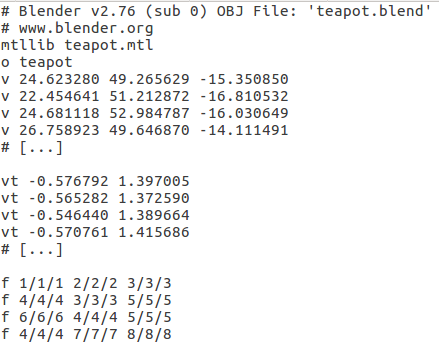
\includegraphics[width=.6\textwidth]{obj_content.png}\\ % PNG-File
  \caption{Notation in .OBJ format}\label{fig:obj_content}
\end{figure}

All these types of information share the following properties which were of relevance for this work. They are contiguous lists of lines, each line representing one instance of the data type indicated in the beginning of the line. Figure \ref{fig:obj_content} depicts an excerpt of an .OBJ file ocntaining vertices (lines starting with v), vertex texture coordinates (lines starting wit vt) and faces (lines starting with f).

These lists are not ordered. Depending on the modelling process, the vertices, faces and all the other attributes can be presented in an completely arbitrary order which hold very little information about the actual, geometric features of the object. The spatial position of any given vertex in relation to the entire object can not be retrieved from this type of notation. This created the demand for spatially indexing of 3D data in the scope this work.

I decided to implement the concept of Octrees \cite{Octree} because of its convenient characteristics as well as prior, personal working experience with \textit{quadtrees}. In an octree, the geometric size of the smallest possible leaf node can be determined in direct relation to the object to be indexed and, at any level, all leafs and nodes will be of the same size. This is highly useful in radius-based proximity-requests for multipl reasons as described in section \ref{sec:addVerticesToSelectionByCoordinates()}.

\begin{figure}[htb]
  \centering
  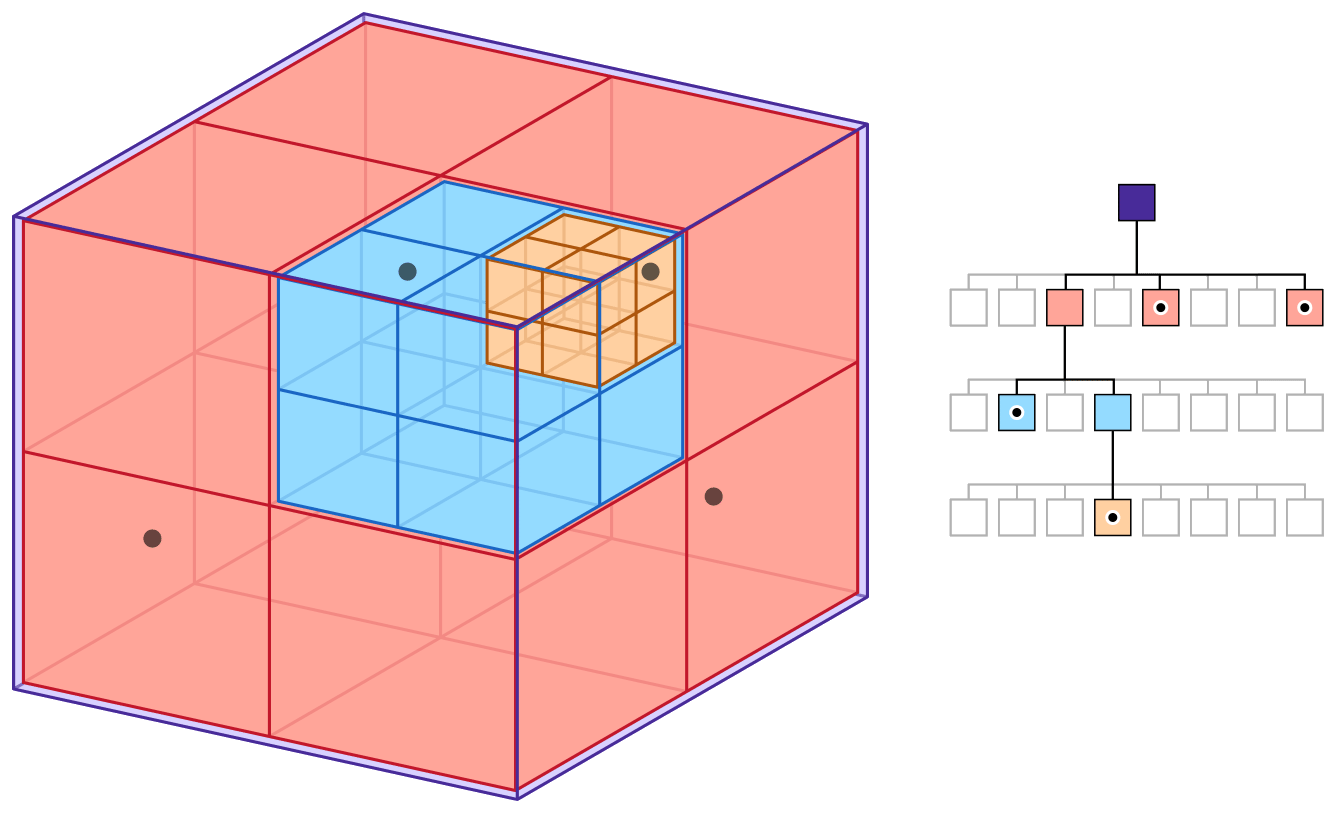
\includegraphics[width=.9\textwidth]{ocTree_apple.png}\\ % PNG-File
  \caption{An octree structure indexing four vertices. Left: 3D view, right: tree structure; 2017, https://developer.apple.com/documentation/}\label{fig:ocTree_apple}
\end{figure}

One of the most common queries performed on 3D data are proximity queries. This means that vertices located within a given radius around an input query-coordinate are to be retrieved. The trivial and obviously highly inefficient solution to such a problem would be to iterate through the entire list of vertices and their coordinates and check for those who fulfill this query condition. This is where spatial indexing structures such ad octree come into play. The concept of octrees is highly recursive and can realize all the most common types of queries (including search queries) in logarithmic time.

An octree is a set of nodes that store references to one another. The highest-level node is called the root node, bottom level nodes are usually referred to as leaf nodes or leafs. Every node that is not a leaf node has eight children-nodes which, in a spatial sense, make up the entire space of their parent node. Such non-leaf nodes can also be described as roots of subtrees.

Figure \ref{fig:ocTree_apple} taken from \cite{octAp} shows a simple octree structure indexing four vertices, both in 3D and tree view. Note how the root node on level 0, shaded purple on the right, is represented as a large purple cube on the left, encompassing the entire set of vertices. The figure clearly visualizes how an non-balanced octree structure that allows one vertex per leaf node at most would look like. On levels 1, 2 and 3, there are eight nodes each. On level 1, there are two leaf nodes that hold one vertex each, on level 2 and 3, there is one leaf holding one vertex.

The most important parameter for an octree is the maximum allowed number of vertices per leaf node. Once the dimensions in x-,y - and z-direction of the 3D object to be indexed have been determined, the root node of the octree will store every vertex until said maximum allowed number of vertices is reached. Up until that point, the root node was still a leaf. It is now a root no longer and will create eight new nodes (its child nodes) and store references to them. This process is repeated recursively for every new node until every leaf node holds less than the maximum allowed number of vertices per leaf node. It is worth mentioning that in many implementations of the octree concept, every leaf node needs to be at the same level. For this work, I decided to implement the non-balanced version of an octree where this is not the case. The reason for this is that in 3D objects, the data is not evenly distributed inside the entire space defined by its bounding box that. The vertices make up the surface of the model, inside and outside of it, there is no spatial information to be indexed at all.

		\subsection{Selection process}
		\label{sec:selection_process}

To gather data to compare with computer generated mesh saliency maps, tracking user input was needed. In the five-sided projection installation of the \cite{v2c}, 3D objects would be loaded and spatially indexed using octrees as described in the section above. Now, the selection function had to be implemented. Using a handheld input device, a so-called \textit{wand}, as depicted in figure \ref{fig:wand}, users can interact with the scene in two essential ways - navigation and performing arbitrary operations mapped to the device's buttons. Each such operation can, among other information, use the current position and rotation of the wand as parameters.

\begin{figure}[htb]
  \centering
  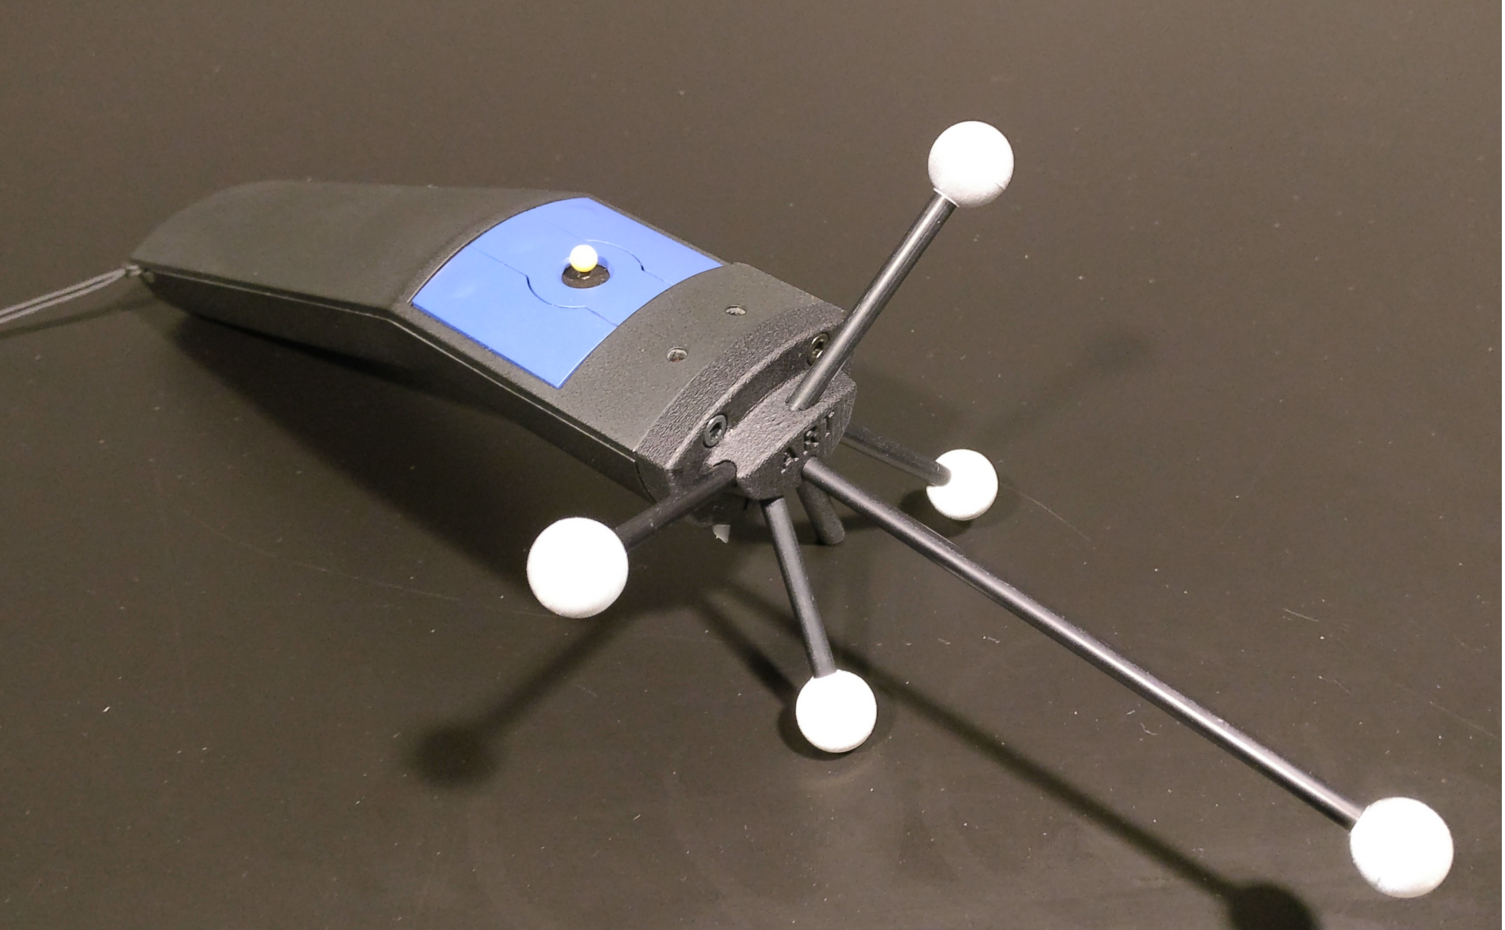
\includegraphics[width=.9\textwidth]{concept_wand.jpg}\\ % PNG-File
  \caption{The input device used at the V2C}\label{fig:wand}
\end{figure}

Figure \ref{fig:wand} depicts the \textit{wand} used in the V2C. The yellow joystick in the middle of its top side, in combination with the current rotation of the device, can be used to navigate the user's view onto the 
scene. The two essential functions of the application are mapped to two of the three buttons surrounding the joystick: The (from the perspective of a user holding the \textit{wand}) left button adds vertices near the current position of the wand to the vertex selection and the righthand button removes such vertices from it. The button in the middle does not have a function in this application, as well as the trigger-like fourth button on the button side of the \textit{wand} (not in view in the figure).
In accordance with the simplistic structure of the user study, the interaction was designed to be as little complex as possible, hence only these two buttons having actual, distinct purposes. 

With this setup in place, everything needed to implement the user selection part of the application is at hand. In order to provide as much visual accuracy as possible, a bright green diamond shaped object at the tracked position of the \textit{wand} is projected into the scene in addition to the loaded model. To additionally provide clear visual feedback, vertices selected are painted in bright red, clearly seperating them from non-selected parts of the object, displayed in plain grey. For more details on the visual presentation of the application, see section \ref{sec:conduct_user_study_with_the_selection_application}.

Whenever a user presses the left button of the \textit{wand}, a proximity query is performed on the octree structure indexing the object with its current position as the input. The position is passed as a \texttt{glm::vec3} variable, a basic 3D vector type provided by openGL's mathematics library. For a detailed description of how such a query is handled in this application, see section \ref{sec:addVerticesToSelectionByCoordinates()}.

In addition to these input coordinates, the following two parameters are passed to calls to this function in the context of a user adding or removing vertices to the current selection. The pre-computed selection radius as a \texttt{float} value and a reference to a temporary set of \texttt{size\_t} values called \texttt{intermediateSelection}, holding unique vertex IDs. After a query is terminated, the set of vertices found will be added to this temporary set.
Due to the design of the synchronisation routine between server and client threads of this application, this set will be emptied before the result of each such query is returend and written to it. If the \textit{add} button was pressed, the content of \texttt{intermediateSelection} will be added to another set holding the list of currently selected vertices total. If the \textit{remove} button was pressed, each of the temporarily selected vertices will be looked up in this second set and, in case it is found, removed from it. This approach prevents the total set of selected vertices to be sent from the server to all client threads at every frame during runtime. Only newly selected vertices (or those that are to be removed from the current selection) are sent across the application. The time for each action (in seconds since the application was started) is logged as well. 

	\section {Conduct user study with the selection application}
	\label{sec:conduct_user_study_with_the_selection_application}
% generell beschreiben (Aufbau, Ziel, Zusammenhang mit vorigen Sections), Details in eigenem grossen Kapitel
Another essential part of this work was conducting a user study where all of the aspects described in this chapter so far would be put to use. The goal was to collect data on what parts of 3D objects users found visually interesting or important. Users put on the stereoscopic, trackable glasses depicted in figure \ref{fig:glasses}, stepped inside the five-sided projection installation of the \cite{v2c} and were asked to mark regions of the object currently displayed that they considered to be intersting or important. The exact wording of the task given to participants in the user study reads as follows.

\textit{Please select parts and regions of the object that}

\begin{itemize}
	\item \textit{you would consider visually interesting or important}
	\item \textit{you would assume are natural focus points of attention}
	\item \textit{are vital for identifying the object}
\end{itemize}

After taking up to five minutes getting familiar with navigating and interaction within the projection installation, as well as selecting and deselecting vertices with the wand (\ref{fig:wand}, the main part of the user study began. 

\begin{figure}[htb]
  \centering
  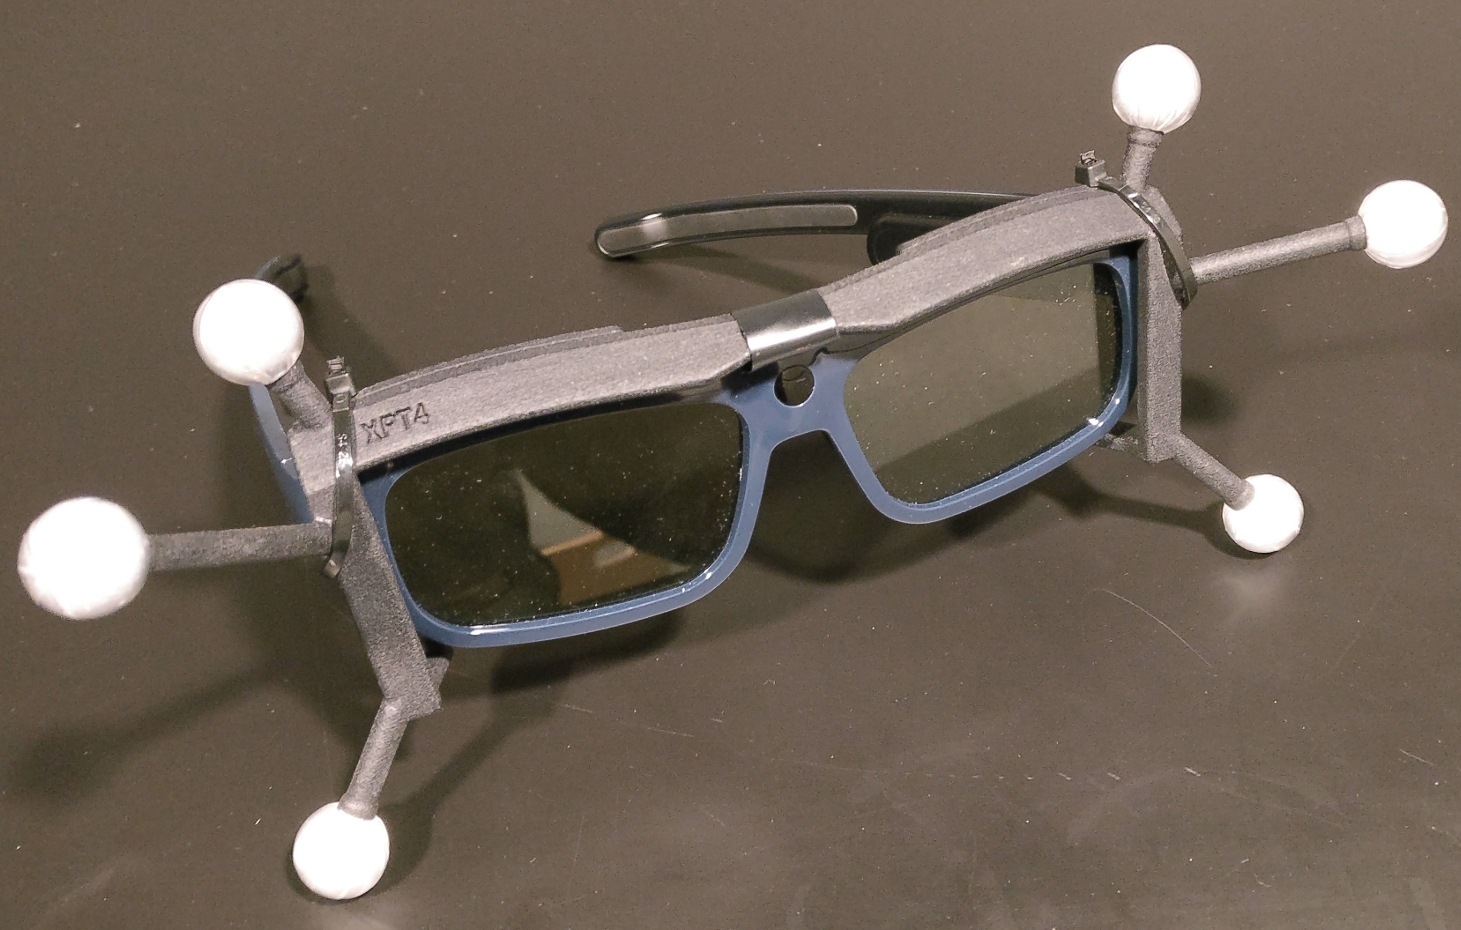
\includegraphics[width=.9\textwidth]{concept_glasses.jpg}\\ % PNG-File
  \caption{The trackable, stereoscopic glasses used at the V2C}\label{fig:glasses}
\end{figure}

Selections of the users would be gathered to compute user-weighted importance maps for the displayed 3D objects. These would be compared to previously computed mesh saliency maps. For the results and discussion of this comparison, see chapter 
% @TODO ref zu chapter "results usw" 1fügen. Selbiges davor noch anlegen

In this selection application, selection and deselection operations are executed with the current tracked position of the \textit{wand} as input coordinates. To give users a clear, live feedback on that tracked position, for every frame, a ten-sided, diamond-shaped object was also rendered in the scene on that very position. The object is shaded in a bright green, to be easily distinguishable within the 3D scene. However, it did not offer a visual representation of the pre-computed selection radius. Again, this radius $r_{max}$ is defined as $d_{min}$ / $2^{l_{max}}$ * 0.95, in other words 95\% the size of the smallest possible leaf node, so it is slightly different for every object loaded in the application. I chose not to adapt the size of the ten-sided object representing the position of the wand and keep it the same size for every object with the intention of providing more consistency within the scene, independent of the currently loaded object. This was also a design decision that went in accordance with the minimalistic general visual presentation of the application, as described in the following brief summary.

\begin{itemize}
	\item background-color of the application: (almost) black
	\item shader used for the loaded object: light grey, no textures, normals used
	\item shader used for selected vertices: bright red
	\item shader used for diamond-shaped object indicating the tracked position of the \textit{wand}: bright green
\end{itemize}

% @TODO: Bild rausrendern (user mit Wand in der Hand, geladenem Object + wand_pos), schneiden und uploaden

Regarding objects used for the study, I aimed at offering as much variety of types of objects among as few objects as possible. The motivation for this was to achieve results that are genereally applicable for any type of geometric data, at least to an basic extent. Also, to avoid the users losing motivation due to repeating tasks during the study, keeping the number of objects to a minimum was another constraint to be considered.
I decided to use three objects described table in \ref{tab:userstudy_objects} and depicted in figure \ref{fig:all_objects}.

\begin{table}[]
\centering
	\begin{tabular}{l|l|l|l|l}
		object	& created through	& source	& vertex count	& class of objects	\\ \hline
		cow	& 3D modelling		& \cite{cow}	& 69,648	& purely natural	\\
		P51 Mustang	&	3D modelling	& \cite{P51}	& 51,708	& purely mechanical	\\
		bunny sculpture	&	3D scan	& \cite{bun}	& 68,754	& natural, man-made	
	\end{tabular}
	\caption{3D objects used in the study}
	\label{tab:userstudy_objects}
\end{table}
% table 3.1

\begin{figure}[htb]
  \centering
  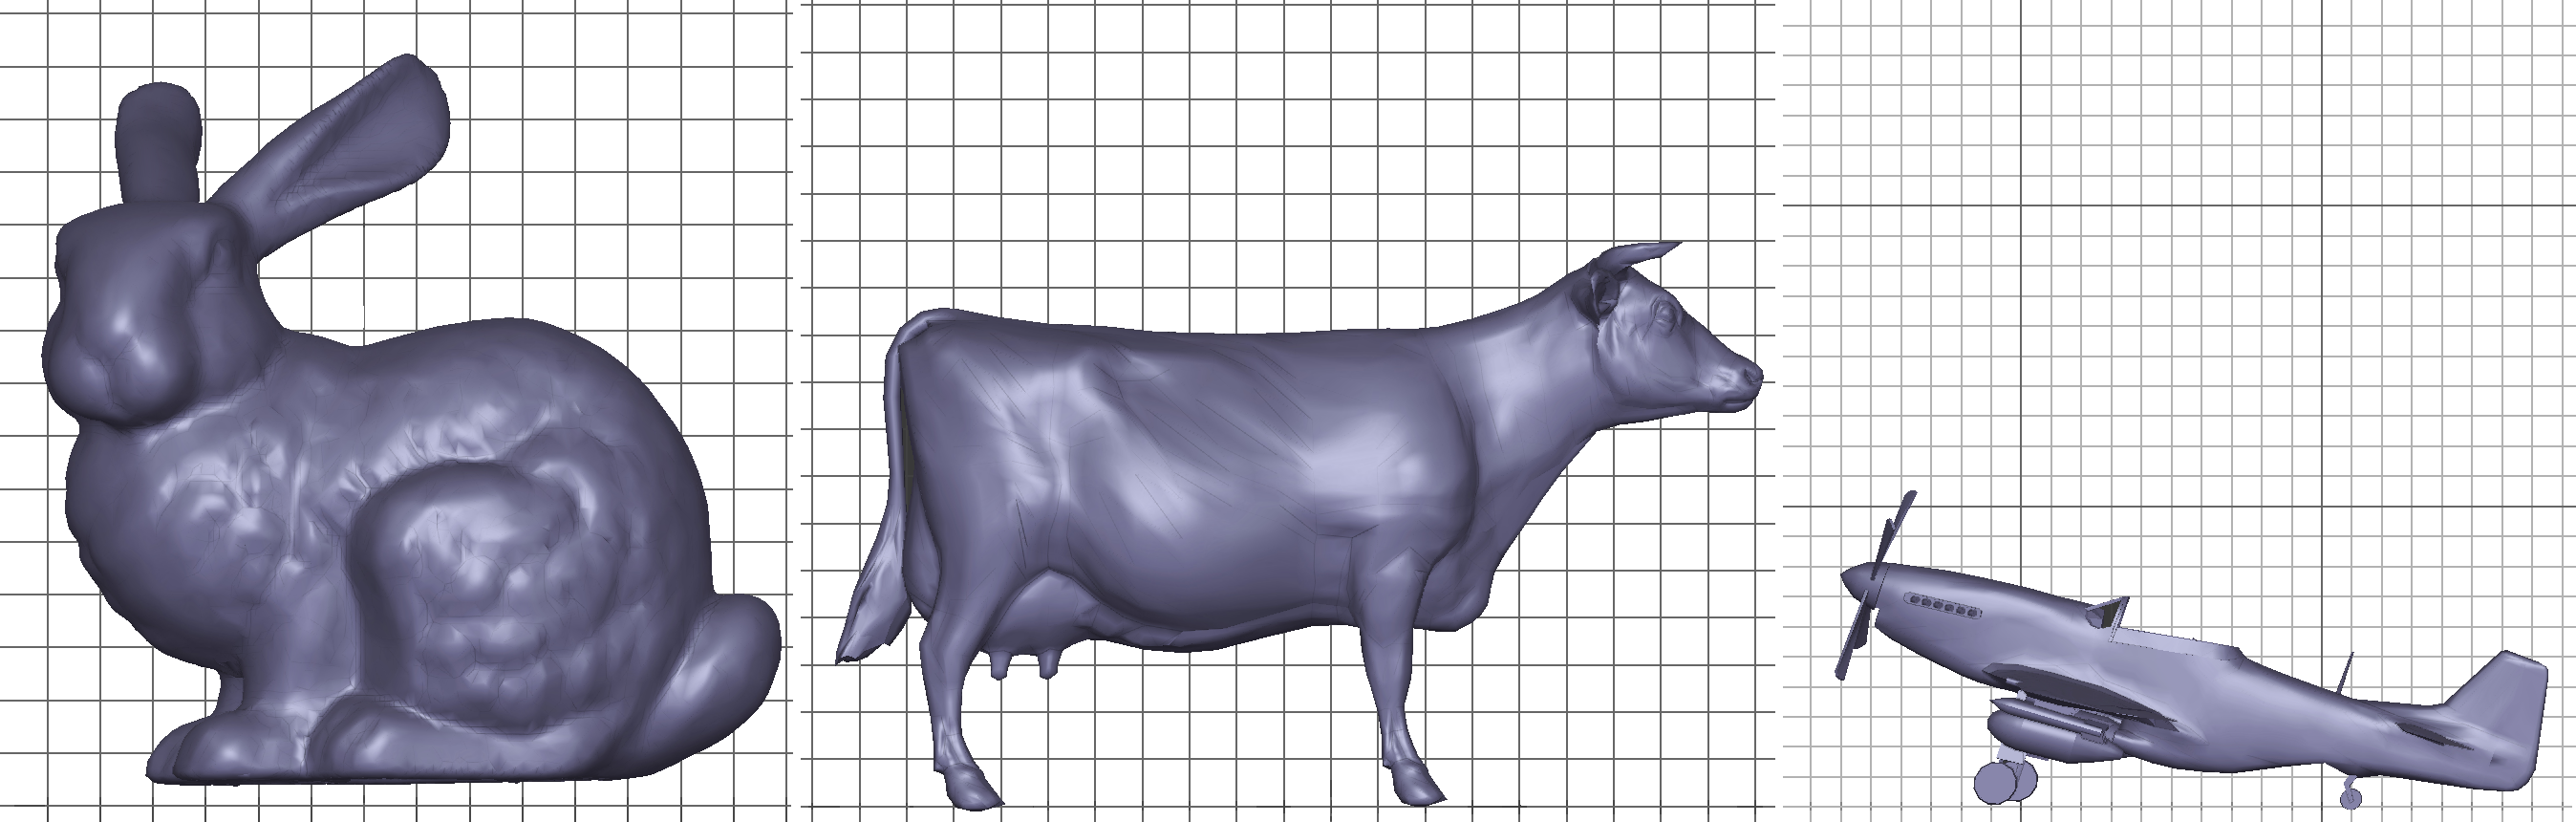
\includegraphics[width=1.0\textwidth]{userstudy_all_objects.png}\\ % PNG-File
  \caption{The 3D objects used for the user study}\label{fig:all_objects}
\end{figure}

Figure \ref{fig:all_objects} shows the objects used in the user study. From left to right, the 3D scanned bunny, the modelled cow and the low-poly, modelled aircraft are shown. Consider the grid to get a sense of their proportions. I did not scale them according to their real world sizes and instead made them take up approximately equal space in the virtual scene. This was done with the intention to provide a similar level of visual detail, independent of the actual geometric level of detail, for each object. Furthermore, I wanted to prevent the size of the objects from having any sort of influence on how users perceived them.

I took two steps to eliminate the possibility of user selections being influenced by them first having to adapt to and getting familiar with the selection application. First, Every user was given five minutes to get familiar with the navigation and selection workflow. Selections made here were not considered for the results of the userstudy. After that, the three objects were presented in a randomly chosen order for five minutes each. The users were given the tasks stated at the beginning of this section and were free to use as much of the five minutes as they wanted to perform vertex selection and deselection operations.

The five minute time limit was an absolute upper limit for each selection process. Users were free to end selection prematurely whenever they stated they were satisfied with the selection as it is.

Besides the five minute \textit{tutorial phase} - the time users could take to get familiar with the application - and the actual tasks to be fulfilled (as described at the beginning of this section), only one more minor request was asked to be considered by users: An approximate symmetrical selection, meaning that, in cases where it was possible, parts of objects users selected on one side of an object would also be selected on the opposite side. Other than that, no additional information or hints were given. Users were told that there is no \textit{correct} way of to fulfill the selection task. They were encouraged to select whatever they deemed relevant according to the tasks based on their personal judgement.

	\section {Measure of differences}
	\label{sec:measure_of_difference}
Since a large portion of the workload of this work was the implementation of the selection application itself, as well as customizing it to the point it is executable in the V2C, the comparison of user generated and pre-computed mesh saliency maps was designed to be quick and easy. In this chapter I will describe how I conceptualised a basic way to compute a \textit{difference ratio}, normalised to a decimal value between 0 and 1, describing how much user saliency maps differ from mesh saliency maps. It is based on a simple vertex-wise comparison of saliency-values and makes use of the proximity queries provided by the octree structure, which is also the basis for the selection application itself as described in section \ref{sec:spatial_indexing_via_octree}.

In chapter % @TODO ref zu chapter "results usw" 1fügen. Selbiges davor noch anlegen
I consider both \textit{raw} and \textit{weighted difference} values, for a detailed explanation of these terms, see the following subsections. For a brief summery and step-wise explanation, see subsection \ref{sec:ste_wise_summery}.

		\subsection{Terms and abbreviations}
		\label{sec:concept_terms_and_abbreviations}
% @TODO threshold einbauen!! Hier und im Quelltext
The following terms, symbols and abbreviations will be used in the subsequent sections to explain the measure of difference used in this work.

\begin{description}
	\item[unweighted difference ratio] - a float number, normalised to a value between 0.0 and 1.0 indicating how much the generated \textit{user saliency map} differs from the pre-computed \textit{mesh saliency map}, based on unweighted (raw) difference values
	\item[weighted difference ratio] - a float number, normalised to a value between 0.0 and 1.0 indicating how much the generated \textit{user saliency map} differs from the pre-computed \textit{mesh saliency map}, based on weighted difference values
	\item[$v_i$] - the currently considered vertex \textit{i} $\in$ set of all vertices $V$ belonging to an object
	\item[$S_{M}(v_i)$] - the computed mesh saliency value for $v_i$ as described in \cite{lee2005mesh}
	\item[$S_{U}(v_i)$] - the user generated saliency value for $v_i$, describing its \textit{perceived importance} value based on how many times it was selected by users in relation to the most-selected vertices.
	\item[$\Delta_{raw}(v_i)$] - the unweighted (raw) difference between the user and mesh saliency values $S_{U}(v_i)$ - $S_{M}(vi_i)$. The absolute value of the result is normalised to a value between 0.0 and 1.0
	\item[$\Delta_{weighted}(v_i)$] - the weighted difference between the user and mesh saliency values $S_{U}(v_i)$ - $S_{M}(vi_i)$. The absolute value of the result is normalised to a value between 0.0 and 1.0
	\item[$V_{proximty}(v_i)$] - a \textit{proximity set} of vertices $v_1$, ... $v_j$ that are located within radius $r$ around the coordinates of given vertex $v_i$
	\item[$\omega$] - a threshold value derived from mesh saliency values $S_{M}(v_1)$, ... $S_{M}(v_j)$ for all vertices $v_1$, ... $v_j$ $\in$ a \textit{proximity set} $V_{proximty}(v_i)$ of $vi$
\end{description}
% @TODO: OMEGA beschreiben, im Quelltext & hier!!! (mit Markus abklären!)

		\subsection{unweighted difference ratio}
		\label{sec:unweighted_difference_ratio}
As stated above, $\Delta_{raw}(v_i)$, or the unweighted (raw) difference between user generated and computed mesh saliency value can easily be obtained by taking the absolute value of $S_{M}(v_i) - S_{U}(v_i)$. For each of the objects used in the user study, we computed a mesh saliency map using \texttt{climberpi's} implementation of \textit{mesh saliency} \cite{clms}, providing $S_{M}(v_i)$ for every vertex $v$ in $V_{bunny}$, $V_{cow}$ and $V_{P-51}$ where $V_{l}$ is the set of all vertices that make up the object with label $l$.

Values $S_{U}(v_i)$ are computed via a simple, average-based comparison of how many users selected each vertex. As mentioned in \ref{sec:user_selection}, user selections are written to simple structured text files containing one unique vertex ID and the time they were added to the selection (in seconds since the application was started) in every line, seperated by a tab symbol as depicted in table \ref{tab:user_selection_log_file}.

\begin{table}[]
\centering
	\begin{tabular}{l|l}
	vertId & timestamp \\ \hline
	27 & 64 \\
	59 & 62 \\
	63 & 62 \\
	64 & 62 \\
	65 & 62 \\
	67 & 62 \\
	68 & 62 \\
	69 & 62
	\end{tabular}
	\caption{Sample content of a user selection log file}
	\label{tab:user_selection_log_file}
\end{table}
% table 3.3

In the simple evaluation tool used for this work, before each logfile is read, a \texttt{std::vector<size\_t, int>} is created with size equivalent to the number of vertices of the currently considered object. After the last log file is processed, this \texttt{set} $userselections$ contains a mapping for each vertex $v_i$, describing how many users selected it with the \texttt{int} value at offset $i$, which equals the vertex ID represented as a \texttt{size\_t} value. In other words, let $userselections[i] = t$ for each vertex $v_i$ of an object where $t$ is the amount of users that selected $v_i$.

Next, the maximum number of times one or multiple vertices were selected $t_{max}$ is computed. Based on this maximum value, \textit{user saliency} values are $S_{U}(v_i)$ generated as follows.

$S_{U}(v_i) = userselections[i]/t_{max}$

\textit{User saliency} values for each of most selected vertices - those selected by $t_{max}$ users - will be 1.0, and 0.0 for those which were not selected by a single user. Every other \textit{user saliency} value will be somewhere in that range, describing what one could informally call the \textit{popularity} of the vertices.

With both \textit{mesh} and \textit{mesh saliency} values for each vertex $v_i$, we can use the absolute value of their difference as the \textit{unweighted (raw) difference}. The final step to generate the overall \textit{unweighted difference ratio} is a simple addition of $S_{U}(v_i)$ values for every $v_i \in V$, where $V$ is the total number of one object and dividing the result by $V$. This ratio gives a quick, first impression of how much the average user selection differs from a \textit{mesh saliency map} computed according to \cite{lee2005mesh}.

		\subsection{weighted difference ratio}
		\label{sec:weighted_difference_ratio}
The unweighted \textit{difference ratio}, being very basic and average based, lacks expressiveness. During research and preparation for this work, it became clear that \textit{mesh saliency maps} offer a solid basis for prediction models of what parts of 3D objects human attention tends to gravitate towards. By further developing and refining the concept, these predictions became precice and reliably, see chapter \cite{sec:related_work}. I based my idea for the \textit{weighted difference ratio} on the assumption that differences in saliency values for some vertices are more interesting than others.

\begin{figure}[htb]
  \centering
  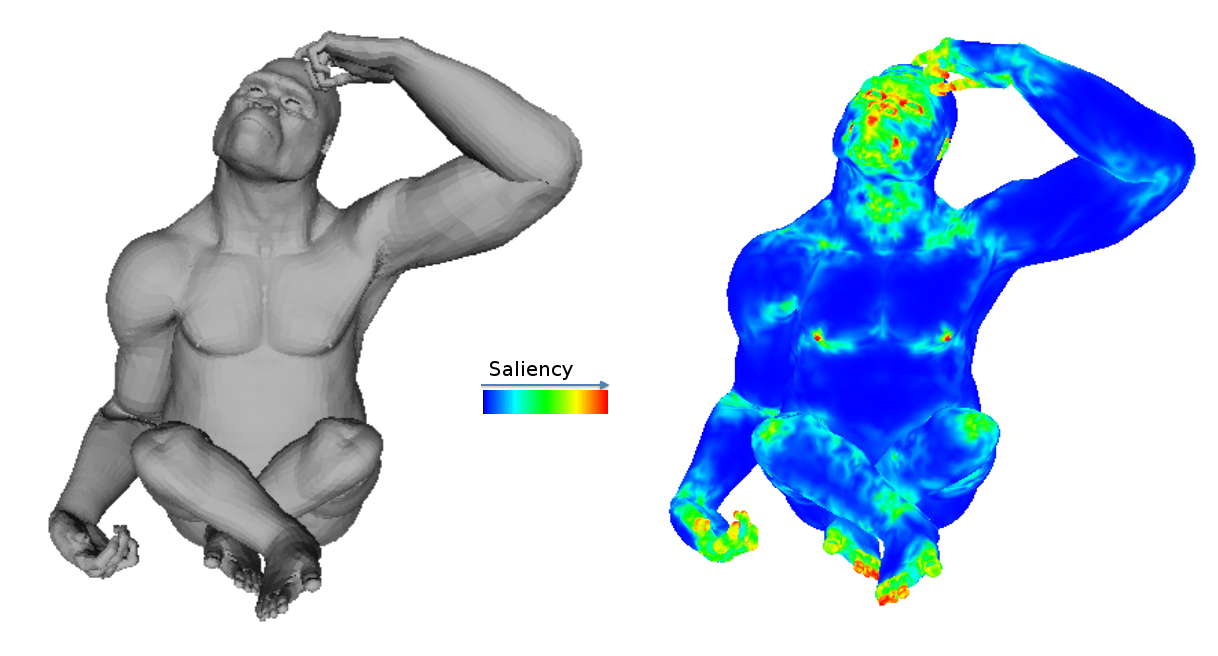
\includegraphics[width=1.0\textwidth]{mss_gorilla_alpha.png}\\ % PNG-File
  \caption{A multi-scale mesh saliency map for an object including color scale. Published by Nouri \textit{et al.} \cite{nouri2015multi}}\label{fig:gorilla_saliency_map}
\end{figure}

Consider figure \ref{gorilla_saliency_map}. It depicts an object and its multi-scale mesh saliency map as well as a scale for reference. The scale describes how yellow and red colored vertices indicate high mesh saliency values for those vertices while green and blue colored ones suggest lower values. Note that this map was not computed via the \textit{standard} mesh saliency model but an enhanced, multi-scale based one. The figure is suitable to explain the idea behind which point-wise difference value in user and mesh saliency values are \textit{weighted} in this work.

Based on the assumption that a very low \textit{user saliency value} of vertices which lays in a yellow or red shaded area is more interesting than one that is located in a green or blue area, I based the decision which vertex-wise difference ratios would be weighted on a comparison of other vertices surroundind them. Consider a vertex $v_i$ in the following cases.

\begin{description}
	\item [case 1:] $v_i$ has a \textit{user saliency} value of 0.2 or lower and vertices in $V_{proximty}(v_i)$ have an average \textit{mesh saliency} value of $\omega$ or higher.
	\item [case 2:] $v_i$ has a \textit{user saliency} value of 0.2 or lower and vertices in $V_{proximty}(v_i)$ have an average \textit{mesh saliency} lower than $\omega$
	\item [case 3:] $v_i$ has a \textit{user saliency} value of 0.8 or higher and vertices in $V_{proximty}(v_i)$ have an average \textit{mesh saliency} value of $\omega$ or higher
	\item [case 4:] $v_i$ has a \textit{user saliency} value of 0.8 or lower and vertices in $V_{proximty}(v_i)$ have an average \textit{mesh saliency} lower than $\omega$
\end{description}

I decided to base this simple evaluation process on the assumption that realistic, reliable results are achieved by the model of \textit{mesh saliency}. So I focused on finding deviations within parts and regions of objects that have higher mesh saliency values. Thus, only in cases 1 and 3, vertex-wise differences get weighted. High vertex-wise differences in regions with a low overall mesh saliency value still are considered for the final \textit{weighted difference ratio}, but not as much as those at hand in cases 1 and 3.
% @TODO: 0.2, 0.8? Hier beschreiben und im Quelltext ggf anpassen (threshold = average_saliency_val oder sowas)
% @TODO: überhaupt checken ob das so stimmt / Sinn ergibt / etc

Regarding how the actual weighting is done, I aimed for a simple function that increases the vertex-wise \textit{raw difference} values, normalising them between 0.0 and 1.0 without getting greater than 1.0. So I chose to use an altered, restricted function describing a circle that has its centre at $x = 1.0, y = 0.0$ and radius $r = 1.0$. Figure \ref{fig:weighting_function} depicts this \textit{weighting function}. It shows how vertex-wise differences between \textit{mesh saliency} and \textit{user saliency} values are used for computation of the final, overall difference ratios - both \textit{unweighted} (black line) and \textit{weighted} (blue curve).

\begin{figure}[htb]
  \centering
  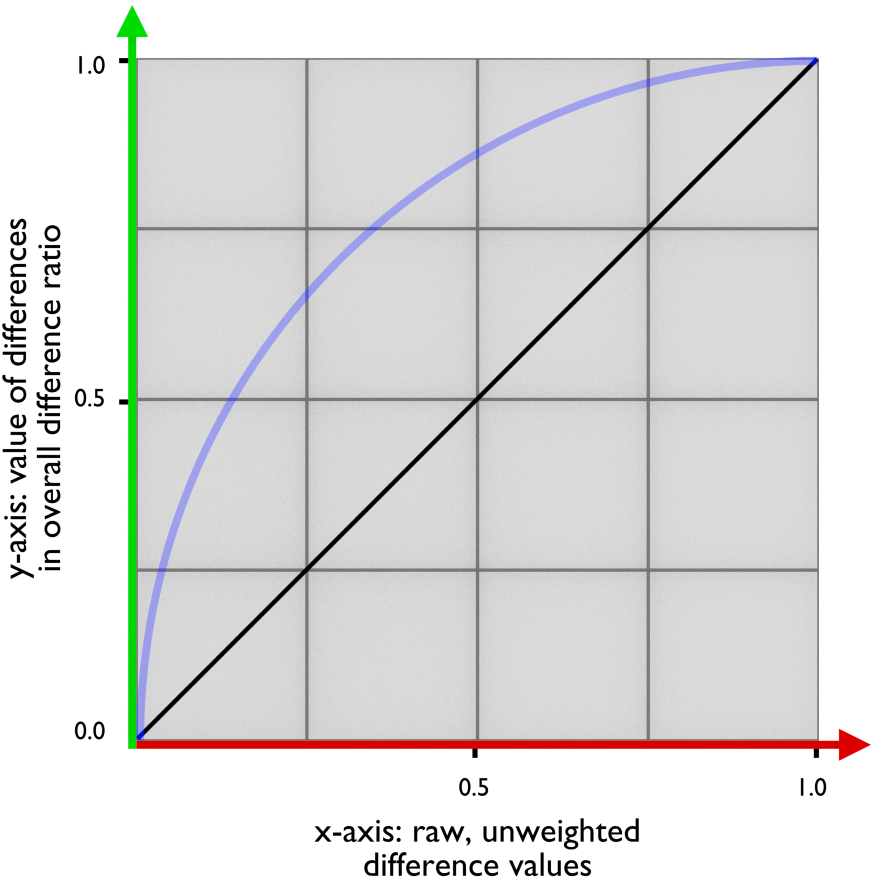
\includegraphics[width=.7\textwidth]{weighting_function.png}\\ % PNG-File
  \caption{Graphic representation of the weighting function in relation to the \textit{unweighted} difference values (straight, black line)}\label{fig:weighting_function}
\end{figure}
% @TODO: blaue Kurva halb-transparent machen

Consider figure \ref{fig:weighting_function}. The straight, black line, being a steady identity function of float values, shows normalised \textit{unweighted} vertex-wise difference values. For such values, both in regards to \textit{unweighted} and \textit{weighted} overall \textit{difference ratios}, their unaltered, absolute value $\Delta_{raw}(v_i)$ is used for computation. However, should vertices in $V_{proximty}(v_i)$ have an average \textit{mesh saliency} value of $\omega$ or greater, the difference between \textit{mesh saliency} and \textit{user saliency} values at $v_i$ is weighted according to the blue curve function shown in the figure.

In conclusion, if $v_i$ is surrounded by vertices whose average of computed \textit{mesh saliency} values surpasses a certain threshold $\omega$, I assume it is located in a greater, contiguous patch of the object with high importance as determined by the processing according to \textit{mesh saliency}. Hence, $\Delta_{raw}(v_i)$ is used for generating the overall \textit{unweighted difference ratio} and $\Delta_{weighted}(v_i)$ is used used for generating the overall \textit{weighted difference ratio}.

		\subsection{step-wise summery}
		\label{sec:ste_wise_summery}
This subsection provides a brief summary of the steps to computing overall \textit{unweighted} and \textit{weighted difference ratios} described in greater detail in the precedig subsections. It provides more insight into how I organised and prepared the data for evaluation. It describes the workflow for a single 3D object.

\begin{enumerate}
	\item Compute the \textit{mesh saliency} map for a given object using using \texttt{climberpi's} implementation \cite{clms} and store the result in an external textfile \texttt{computed\_saliency} for later use.
	\item Read \textit{n} textfiles \texttt{u\_00}, ... \texttt{u\_n}, each containing one user selection, compute the \textit{user saliency} map based on how many times each vertex was selected in relation to the most-selected vertices and store the result in an external textfile \texttt{user\_saliency} for later use.
	\item Read \texttt{computed\_saliency} and \texttt{user\_saliency}, store the contents in two \texttt{std::vector} containers \textit{computed\_saliency\_values} and \textit{user\_saliency\_values}.
	\item calculate vertex-wise saliency differences and store them in an a \texttt{std::vector differences\_unweighted}.
	\item Iterate through the list of vertices of the currently considered object. For every such vertex $v_i$, find vertices $v_1$, ... $v_j$ $\in$ $V_{proximty}(v_i)$ via a range-query to the \texttt{ocTree} instance indexing the object (see section \ref{sec:addVerticesToSelectionByCoordinates()}).
	\item For each vertex $v_i$, look up \textit{mesh saliency} values for vertices $v_1$, ... $v_j$ in the \textit{mesh saliency} map. Compute the average of those values.
	\begin{enumerate}
		\item if average is $\omega$ or greater, compute $\Delta_{weighted}(v_i)$ and storte it in a \texttt{std::vector differences\_weighted}.
		\item if average is less than $\omega$, keep $\Delta_{raw}(v_i)$ as it is in \texttt{differences\_unweighted}.
	\end{enumerate}
	\item Iterate through \texttt{differences\_unweighted}, calculate the average and return it as the overall \textit{unweighted difference ratio}.
	\item Iterate through \texttt{differences\_weighted}, calculate the average and return it as the overall \textit{weighted difference ratio}
\end{enumerate}


	\chapter{Selection Application}
\label{sec:selection_application}

This chapter describes the of the selection application used for this work. After a rundown of third party requirements and a summary of relevant C++ classes, the description is further subdivided according to its abstract, key requirements.
The goal of this chapter is to describe how the application, especially the ctree\cite{Octree}, is designed and implemented. Accordingly, key lines of source code as well as plenty of explanatory comments are provided.

\section{Additional third party libraries}
\label{sec:additional_third_party_libraries}
To ensure a scalable, platform independent implementation of the application, the following third party libraries, frameworks and APIs are used.

\subsection{Mesh saliency by climberpi}
\label{sec:mesh_saliency_by_climberpi}
A student at Zhejiang University \cite{zju} has implemented the concept of \textit{mesh saliency} following the original paper by Lee \textit{et al.} This implementation is written in C++ and available at \cite{clms}. It is of vital importance to this work, as \textit{mesh saliency} maps are computed using this piece of software.

\subsection{OpenGL}
\label{sec:opengl}

The Open Graphics Library OpenGL \cite{OpenGL} is a powerful industry standard API for rendering 2D and 3D graphics, independently of programming language and operating system. One of its most outstanding features is its ability to directly perform operations on the graphics processing unit of a computer, allowing fast, hardware-accelerated display of graphic elements. For this work, OpenGL is used for displaying the 3D objects both in the user study and throughout development of the selection application. The task of displaying rendered images across multiple projection surfaces on a 360\degree panorama view is handled by software developed at the Zentrum f\"ur Virtuelle Realit\"at und Visualisierung (V2C) of the Leibniz-Rechenzentrum \cite{v2c}.

OpenGL is based on the following basic structures and concepts:

\begin{description}
	\item[Vertex Buffer Objects] (VBOs) contain actual vertex data. Coordinates, normal and color information, texture mapping and any other kind of data that is desired can be saved in these kinds of objects. They are designed as buffer objects to be stored directly within the memory of the video card, ensuring extremely fast access times.
	\item[Vertex Array Objects] (VAOs) are objects which can contain one or more Vertex Buffer Objects and store information for complete, rendered objects. In other words, VAOs store descriptions of vertex data stored in VBOs. For example, the number of coordinates the vertices are made of, in which order etc. From a performance aware point of view, they are a great improvement over older, deprectecated concepts in OpenGL since multiple calls to bind and upload distinct sets of data belonging to the same object to the graphics processing unit can be bundled in one call to a VAO.

	\item[Vertex Shaders] are small pieces of C-like code, executed by the graphics card, which can perform extremely fast, basic operations on every vertex of a vertex data input stream. Vertex shaders are one of two mandatory types of shaders. As soon as an openGL \texttt{draw} command is called, they process every incoming vertex and output two things for each one: Its position (untouched or altered in any way desired) within the output window on screen, and a set of arbitrary defined custom data such as normal information, color and texture mapping. These attributes are calculated on a per-vertex basis.

	\item[Fragment Shaders] complete the absolute minimum for an openGL-based rendering pipeline to be able to display anything, together with vertex shaders. They are executed per pixel and, therefore, potentially a lot more times than vertex shaders. Their purpose is to interpolate, for each pixel in between vertices, its RGB value, based on the per-pixel values calculated by the vertex shader. The term \textit{fragment} is often informally described as a \textit{potential pixel}, as the final RGB value of a pixel can still be changed after it is processed by the fragment shader.

\end{description}

\subsection{GLUT}
\label{sec:glut}

As stated on its official webpage \cite{GLUT}, GLUT is an official OpenGL Utility Toolkit which provides, among other features, support for multiple windows, control of such windows and handling input from devices such as keyboards and mouses. It is commonly used to achieve interactive windows with cross-platform compatibility displaying rendered images produced by OpenGL. Handling input via the hand-held controller in the user study is achieved with the help of GLUT during this work.

\subsection{GLEW}
\label{sec:glew}

The OpenGL Extension Wrangler Library (GLEW)\cite{GLEW} is a cross-platform extension loading library, specifically designed to be used by C/C++ applications. It provides run-time mechanisms for OpenGL extensions supported on the target platform, allowing to faster query and load those extensions.

\subsection{ASSIMP}
\label{sec:assimp}

Available across multiple operating systems including Android and iOS, The Open Asset Import Library \cite{ASP}, is a powerful open source library that offers import, export and post-processing functions for most commonly used 3D data formats. In this work, its easy to use import function for OBJ files is used for loading the 3D objects to be displayed in the user study. ASSIMP implements a set of hierarchically organised data structures or so-called nodes. Two of the most relevant ones for this work are briefly described below.

\begin{description}
	\item[aiScene] is the root of all the imported data returned from a successful call to one of ASSIMP's import functions. Global information such as the direction of the coordinate system, its origin location as well as references to all the other data in the scene are stored here.
	\item[aiMeshes] represent imported meshes within the scene. Each aiMesh has its own local coordinate system with an origin point and all the vertices belonging to it. Multiple sets of data describing one imported mesh can be stored in these mesh objects but sets of vertices and faces are always guaranteed to be present, thus enabling a basic graphic representation of the mesh.
\end{description}

\section{Relevant class files}
\label{sec:relevant_class_files}

This section covers all the relevant C++ classes used to implement the selection application. Note that these descriptions only cover the general structure and purpose of these classes within the context of the applicatoin. For a more detailed description of the most crucial functions, see section \ref{sec:key_features}.

\subsection{Object}
\label{sec:object}

The object class is used to represent a 3D object within the project. It uses import functions from ASSIMP to load a file via a given source path. An object can contain multiple mesh objects, segmentation happens automatically based on a threshold number of vertices that can be stored in one mesh. This class is used to work with potentially very large 3D files in a uniform and quick way, mostly by implementing wrapper functions that have each mesh object associated to an object call their upload and draw functions, their destructors etc.

\subsection{Mesh}
\label{sec:mesh}

One object can consist of multiple meshes. These meshes are coherent with instances of aiMesh (see subsection \ref{sec:assimp}) and all the important attributes such as vertices, faces, normals, texture coordinates and IDs are stored here. OpenGL functions such as uploading vertex buffer data to the graphics proccessing unit and drawing are implemented here. Some of the application's most crucial functionalities such as adding to and removing vertices from the global selection of vertices to be highlighted are implemented in this class, see \ref{sec:key_features}.

\subsection{Octree}
\label{sec:octree}
Spatial indexing of loaded objects in the application is entirely handled in this class. This has been one of the most labour-intensive parts of the application because formal guides to implementing it, independent of coding language, are scarce and working with the data that is stored in the object and mesh classes above required an extensive amount of customisation.

\section{Key Features}
\label{sec:key_features}
This section describes the following features and functionalities which are most crucial to the selection application.

\begin{itemize}  
	\item Spatial indexing via Octree
	\item User selection
	\item Tracking selection
	\item Testing setup 
\end{itemize}

\subsection{Spatial indexing via Octree}
\label{sec:spatial_indexing_via_octree}

As mentioned above, the \texttt{ocTree} class handles spatial indexing and, therefor, provides quick access to every vertex of an imported 3D object via a set of integer-like (\texttt{size\_t}) indices. The general approach to this implementation of the concept of octree is designed with a heavy emphasis on its recursive features. Instances of it can be created from everywhere in the application by the call of its public root constructor function. Nodes can be leafs or not, which is indicated by a boolean flag for every instance of an \texttt{ocTree} object. Leaf nodes do not have subtree-nodes that refer to them as parents, they solely store vertices within their bounds. Non-leaf nodes have eight children nodes, in other words, eight more \texttt{ocTree} objects which refer to them as their parent node.

For better understanding during development and clearer, human-readable log messages, unique binary identifiers were implemented with care. Each node of the tree has a private \texttt{std::vector} which serves as a unique combination of boolean values describing its identifier. It can be used for directly accessing any desired \texttt{ocTree} (subtree) object within a tree through its root node.

Starting from the root node (level \textit{l} = 0), such an identifier \textit{Id} with a length of \textit{n} boolean values can be used for locating the respective node within 3D space by considering three of its consecutive values at a time. At any level \textit{l}, those  values of \texttt{Id} can be found at positions \textit{$O_l$}, \textit{$O_l$+1} and \textit{$O_l$+2} within it, where $O_l$ is the \textit{level offset} $l*3-3$. If \textit{$O_l$+2} equals its length \texttt{n}, the search ends and the resulting node can be queried for the vertices within its bounds. Every non-leaf node has eight subtree nodes on level \textit{l+1} where \textit{l} is the level of that node. Their bounds can be derived directly from the parent nodes' maximum and minimum values as table \ref{tab:child_node_bounding_values} depicts. The suffix \textit{p} for new values refers to the parent node, \texttt{[n]} is the \texttt{n}th element of identifier \texttt{ID}. $O_l$ describes the \textit{level offset} $l*3-3$. Note that \texttt{$O_l+3$} determines the child node's minimum and maximum values in x, \texttt{$O_l+2$} in y and \texttt{$O_l$} in z dimension.

\begin{table}[]
\begin{tabular}{l|llllll}
Id{[}$O_l$, $O_l$+1, $O_l$+2{]} & X min & X max & Y min & Y max & Z min & Z max \\ \hline
000 & \textit{p}.X min & \textit{p}.X mean & \textit{p}.Y mean & \textit{p}.Y max & \textit{p}.Z mean & \textit{p}.Z max \\
001 & \textit{p}.X mean & \textit{p}.X max & \textit{p}.Y mean & \textit{p}.Y max & \textit{p}.Z mean & \textit{p}.Z max \\
010 & \textit{p}.X min & \textit{p}.X mean & \textit{p}.Y min & \textit{p}.Y mean & \textit{p}.Z mean & \textit{p}.Z max \\
011 & \textit{p}.X mean & \textit{p}.X max & \textit{p}.Y min & \textit{p}.Y mean & \textit{p}.Z mean & \textit{p}.Z max \\
100 & \textit{p}.X min & \textit{p}.X mean & \textit{p}.Y mean & \textit{p}.Y max & \textit{p}.Z min & \textit{p}.Z mean \\
101 & \textit{p}.X mean & \textit{p}.X max & \textit{p}.Y mean & \textit{p}.Y max & \textit{p}.Z min & \textit{p}.Z mean \\
110 & \textit{p}.X min & \textit{p}.X mean & \textit{p}.Y min & \textit{p}.Y mean & \textit{p}.Z min & \textit{p}.Z mean \\
111 & \textit{p}.X mean & \textit{p}.X max & \textit{p}.Y min & \textit{p}.Y mean & \textit{p}.Z min & \textit{p}.Z mean
\end{tabular}
\caption{Child node bounding values}\label{tab:child_node_bounding_values}
\end{table}
% table 4.1

The most important functions of the \texttt{ocTree} class, as implemented in this work, are described below.

\subsubsection{Root constructor \texttt{ocTree()}}
\label{sec:root_constructor}
	This public constructor creates a new instance of the class \texttt{ocTree}. Parameters required are
	\begin{enumerate*}
		\item a sequence container, such as an array (\texttt{std::vector} is used in this work) holding the \texttt{mesh} objects to be spatially indexed,
		\item an integer determing the maximum amount of vertices that one leaf node can store, and
		\item an integer determing the maximum split depth, in other words the maximum depth of the tree
	\end{enumerate*}.
	As an optional fourth parameter, a boolean flag can be passed as well. Its default value is set to be \texttt{false}, if it is set to \texttt{true}, additional information regarding the recursive construction of the tree, including identifiers, level, dimensions and number of vertices held by each subtree, are printed to the console via \texttt{std::cout}. During subsequent creation of subtrees, this parameter are used for each new object.

From the main class, for example, creating a new instance of an \texttt{ocTree} object is handled by the following short command:

\begin{minipage}{\linewidth}
\begin{lstlisting}[language=C++,numberstyle=\zebra{black!5}{white}{},numbers=left,xleftmargin=2em,tabsize=3]
myOcTree = new ocTree(meshes, 100, 4, true);
\end{lstlisting}
\end{minipage}

This creates a spatial indexing structure for the 3D data stored in \texttt{meshes} where each node can hold up to 100 vertices and the maximum level of nodes is 4. Additional information is printed to the console because the last parameter is set to \texttt{true}.

\subsubsection{Subtree constructor \texttt{ocTree()}}
\label{sec:subtree_constructor}
	This somewhat more complex, private constructor is used for every \texttt{ocTree} object that is not a node. In addition to the parameters that were used for the root node, the following parameters are required:
	\begin{enumerate*}
		\item A set of vertices to be searched through for those located within the bounds of this particular subtree (\texttt{std::vector} of \texttt{glm::vec3} objects is used in this work), 
		\item An integer determing the level of the parent node, the level of this new subtree is set to that level plus one,
		\item An array of nine float values describing its parents dimensions (together wit the \textit{split directions}, this is used to determine the bounds, or dimensions, of this new subtree),
		\item A reference to the root node of this subtree,
		\item A vector of boolean values describing its parents unique identifier, and
		\item A vector of three boolean values describing the \textit{split directions} passed by the parent node
	\end{enumerate*}.
	Again, an additional boolean flag determing whether, during the recursive building proccess of the subtree, information is printed to the console or not, is also passed with the value of the respective member variable of the parent node.

The crucial task of setting the right unique identifier of a newly created subtree node is also handled in this constructor. The following code-snippet shows how that is implemented in this work.

\begin{minipage}{\linewidth}
\begin{lstlisting}[language=C++,numberstyle=\zebra{black!5}{white}{},numbers=left,xleftmargin=2em,tabsize=3]
ocTree::ocTree(...) {
	int identifierSize = m_parentIdentifier.size();
	int levelOffset = m_level*3-3;
	std::vector<bool> id(identifierSize);

	for (int i = 0; i < levelOffset; i++) {
		id[i] = parId[i];
	}

	id[levelOffset] = splitDirections[0];
	id[levelOffset+1] = splitDirections[1];
	id[levelOffset+2] = splitDirections[2];

	for (int j = levelOffset+3; j < identifierSize; j++) {
		id[j] = false;
	}
	m_identifier = id;
}
\end{lstlisting}
\end{minipage}

After setting up the essential variables, lines 6 - 8 copy the parts of the parent's identifier up until the current level offset. Every new subtree node is a child of a lower-level node and this step implicitly entails that relationship. If an \texttt{ocTree} object at a level higher than 0 has child nodes - which makes it the root of a subtree within the octree - has the unique identifier 010000, the first three values of the identifiers of its eight children nodes is 010.

Lines 10 - 11 set the crucial values at the level offset $O_l$, $O_l+1$ and $O_l+2$ according to the values passed via \texttt{splitDirections}. In the context of a parent node calling \texttt{split()}, these passed values are eight sets of three boolean values each that can be represented as 000, 001, 010, 011, 100, 101, 110 and 111.

Since every identifier of every node within an octree, in this implementation, has to have the same length (that is $3*maximumLevel$ where \textit{maximumLevel} is the maximum allowed level of subtree nodes), lines 14 - 16 take care of assigning \texttt{false} as placeholders to every position that is not relevant due to the node's level. In line 17, the final identifier of the current node is set as its private member variable.

	\subsubsection{\texttt{getRootDimensions()}}
	\label{sec:getRootDimensions}
This is called by a newly created root \texttt{ocTree}. In this first basic step, all vertices of every passed \texttt{mesh} object are iterated through to find maximum values which are used as its general bounds in x, y and z direction. For convenience, a margin value of 0.0001 is added to maximum values and subtracted from minimum values to enable one common rule of unambiguously assigning any given vertex (expecially the ones that are located on boundaries of subtrees) to exactly one subtree - for the root node as well as all subtree nodes.

	\subsubsection{\texttt{setDimensions()}}
	\label{sec:setDimensions}
	\label{sec:setDimensions}
This simple private function takes care of setting up correct minimum, mean and maximum values in x, y and z dimension for a newly created subtree node. The following parameters are required:
\begin{enumerate*}
	\item An array of nine \texttt{float} values containing the parent nodes' bounding and mean values, and
	\item A reference to an \texttt{std::vector} of three boolean values containing the \textit{split directions}
\end{enumerate*}.

Based on the \textit{split directions} given via the second parameter, setting up the bounding values for the new subtree is a matter of assigning the correct value of the first parameter. Said second parameter - a vector of \texttt{float} values - contains its values in the following order:
\begin{enumerate*}
% \setcounter{enum}{0}
\addtocounter{enumi}{-1}
	\item minimum X,
	\item maximum X,
	\item mean X,
	\item minimum Y,
	\item maximum Y,
	\item mean Y,
	\item minimum Z,
	\item maximum Z,
	\item mean Z
\end{enumerate*}.

To convey the idea of what this function does more clearly, consider figure \ref{fig:child_node_000_101.png}. Keeping in mind the order in which the three boolean values that make up \textit{split directions} are handled in the code-snippet below, it is clear that, say for newly created subtree nodes with identifiers 000 and 101 \textit{$N_0$} and \textit{$N_5$}, its bounding and mean values are directly derived from the values of their common parent node \textit{p} as shown in Table \ref{tab:bounding_values_subtree_nodes}.

\begin{minipage}{\linewidth}
\begin{lstlisting}[language=C++,numberstyle=\zebra{black!5}{white}{},numbers=left,xleftmargin=2em,tabsize=3]
void ocTree::setDimensions(...) {
	if (splitDirections.at(0) == false) {
		m_minZ = parentDimensions[8];	// minZ = p.meanZ
		m_maxZ = parentDimensions[7];	// maxZ = p.maxZ
	} else {
		m_minZ = parentDimensions[6];	// minZ = p.minZ
		m_maxZ = parentDimensions[8];	// maxZ = p.meanZ
	}

	if (splitDirections.at(1) == false) {
		m_minY = parentDimensions[5];	// minY = p.meanY
		m_maxY = parentDimensions[4];	// maxY = p.maxY
	} else {
		m_minY = parentDimensions[3];	// minY = p.minY
		m_maxY = parentDimensions[5];	// maxY = p.meanY
	}

	if (splitDirections.at(2) == false) {
		m_minX = parentDimensions[0];	// minX = p.minX
		m_maxX = parentDimensions[2];	// maxX = p.meanX
	} else {
		m_minX = parentDimensions[2];	// minX = p.meanX
		m_maxX = parentDimensions[1];	// maxX = p.maxX
	}

	m_meanZ = (m_minZ+m_maxZ)/2;
	m_meanY = (m_minY+m_maxY)/2;
	m_meanX = (m_minX+m_maxX)/2;
}
\end{lstlisting}
\end{minipage}

\begin{table}[]
\begin{tabular}{l|llllll}
child node & minX & maxX & minY & maxY & minZ & maxZ \\ \hline
\textit{$N_0$} & \textit{p}.minX & \textit{p}.meanX & \textit{p}.meanY & \textit{p}.maxY & \textit{p}.meanZ & \textit{p}.Z max \\
\textit{$N_5$} & \textit{p}.meanX & \textit{p}.maxX & \textit{p}.meanY & \textit{p}.maxY & \textit{p}.minZ & \textit{p}.meanZ \\
\end{tabular}
\caption{bounding values of subtree nodes according to \texttt{setDimensions()}}\label{tab:bounding_values_subtree_nodes}
\end{table}
% table 4.2

	\subsubsection{\texttt{split()}}
	\label{sec:split}
This private function, called by a leaf node in case there are more vertices within its bounds than the maximum number of allowed vertices per leaf, takes care of turning a leaf node into a intermediate node, the root of a subtree in other words. The vertices that are stored by the calling node when this function is called, make up the set of vertices to check by its eight children nodes. These eight subtree \texttt{ocTree} objects are created via a call to the private constructor of the \texttt{ocTree} class. To illustrate the purpose this function serves, the following simplified C++ code-snippet shows the necessary steps for the creation of two of the eight new subtree nodes that are to be constructed.

\begin{minipage}{\linewidth}
\begin{lstlisting}[language=C++,numberstyle=\zebra{black!5}{white}{},numbers=left,xleftmargin=2em,tabsize=3]
bool ocTree::split() {
	float parDimensions[9] = {
		m_minX,	m_maxX,	m_meanX,
		m_minY,	m_maxY, m_meanY,
		m_minZ, m_maxZ, m_meanZ
	};

	std::vector<bool> split0 = {false, false, false};	// 000
	std::vector<bool> split1 = {false, false, true};	// 001
	// <repeat for six remaining bool vectors>

	ocTree* chidlLeaf0 = new ocTree(m_verticesInBounds, m_level,
		m_maxVerticesPerNode, m_maxSplitDepth, parDimensions,
		m_root, m_identifier, split0, m_debugInfo);
	ocTree* chidlLeaf1 = new ocTree(m_verticesInBounds, m_level,
		m_maxVerticesPerNode, m_maxSplitDepth, parDimensions,
		m_root, m_identifier, split1, m_debugInfo);
	// <repeat for six remaining ocTree objects

	m_myChildren[0] = chidlLeaf0;
	m_myChildren[1] = chidlLeaf1;
	// <assign six remaining children to private array of ocTree nodes>

	m_isLeaf = false;
}
\end{lstlisting}
\end{minipage}

Lines 2 - 5 define an array of \texttt{float} values which contains minimum, mean and maximum values in x, y and z dimension for this node. Depending on the so-called \textit{split directions} given via \texttt{split0}, \texttt{split1} and so on, the children nodes of this node is able to retrieve their spatial bounding values directly from \texttt{parDimensions}.

Lines 8 and 9 show the first two vectors of \textit{split directions}. The remaining six (not shown here) go on to describe values 010, 011, 100, 101, 110 and 111.

Lines 12 - 14 and 15 - 17 show the initialisations of two new \texttt{ocTree} objects using the class' private subtree constructor. Note that the two shown calls differ only in one parameter, \texttt{split}\textit{n}. This is also true for the remaining six (not shown) objects to be constructed.

Lines 20 and 21 show the assignments of newly created subtree nodes to their place in the current node's private array of pointers to \texttt{ocTree} objects - its children nodes. This provides fast and direct access to them for later queries. 

	\subsubsection{\texttt{getNodeByIdentifierArray()}}
	\label{set:getNodeByIdentifierArray}
This recursive, public function returns a pointer to a leaf node via a boolean input vector representing its identifier. Starting at the root node, it traverses through tree and returns the node with given identifier at the lowest level. The only parameter required is a \texttt{std::vector} \textit{Id} of \textit{n} = \textit{L}*3 boolean values where \textit{L} is the maximum level of the \texttt{ocTree} object calling this function.

As described above, a node at level \textit{l} that is recursively calling this function, first calculates the current level offset $O_l = l*3-3$ and then considers elements $O_l, O_l+1$ and $O_l+2$ of passed identifier vector \textit{Id}. Depending on these values, the matching child node performs the next recursive call of \texttt{getNodeByIdentifierArray()}. Every \texttt{ocTree} object has a private array as a member variable that holds eight other \texttt{ocTree} objects, its children nodes. Given the bounds of a parent node, which are defined as minimum and maximum values in x, y and z direction, calculating the three mean values in all three dimensions is trivial. The resulting  set of minimum, maximum and mean values can be combined in multiple ways and used for minimum and maximum values of all eight subtree nodes, see table \ref{tab:child_node_bounding_values}. To geometrically locate the children nodes, one must check the three relevant boolean values and search either before or beyond the median values in x, y and z direction. A \texttt{false} value of x means the respective child node lies within the parent node's minimum and mean values in x direction, \texttt{true} means it lies within mean and maximum x values. This pattern is inverted in directions y and z. In both cases, \texttt{false} means the child node starts at the mean value of the parent node (its minimum value equals the mean value of the parent) and ends at its maximum value, whereas \texttt{true} indicates the opposite. Figure \ref{fig:child_node_000_101.png} depicts two exemplary parent nodes at level \textit{l} (checkered) and their bounds with one of their eight subtree nodes, the ones indicated by \textit{Id}[$O_l$, $O_l+1$, $O_l+2$], highlighted in red. Again, note that \texttt{$O_l+3$} determines the bounds in x, \texttt{$O_l+2$} in y and \texttt{$O_l$} in z direction.

\begin{figure}[htb]
  \centering
  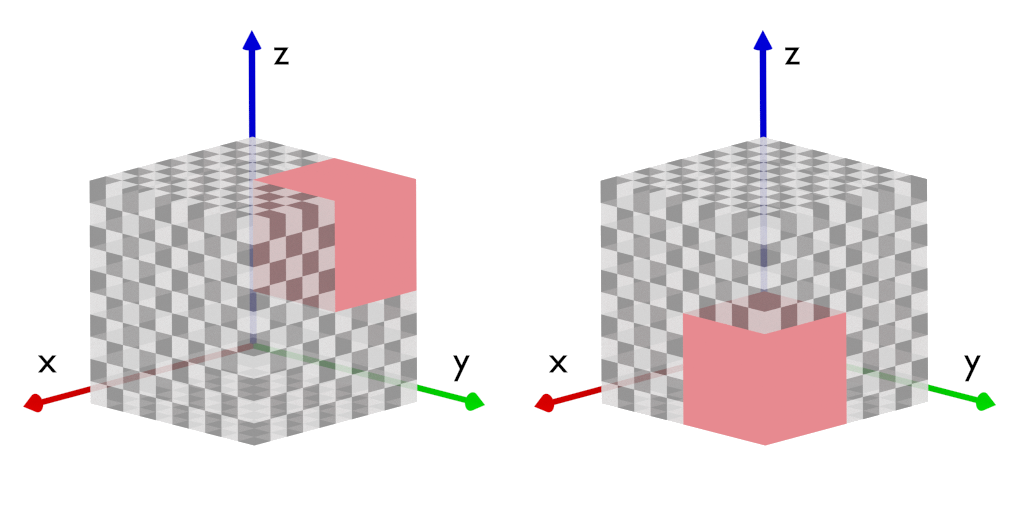
\includegraphics[width=.8\textwidth]{child_node_000_101.png}\\ % PNG-File
  \caption{Parent node (checkered) highlighted child nodes. Left: 000, right: 101}\label{fig:child_node_000_101.png}
\end{figure}

	\texttt{getNodeByIdentifierArray()} returns a reference to an \texttt{ocTree} object whose identifier matches the series of boolean values passed during the call. It mainly served testing and debugging purposes during development of the application, making sure the spatial indexing structure would be computed correctly for any given set of input 3D data. It is a utility function that provides fast, direct acces to any one desired node within an \texttt{ocTree} structure.

	\subsubsection{\texttt{buildTreeRecursively()}}
	\label{sec:buildTreeRecursively}
A call to this function causes an entire set of given vertices to be indexed and assigned leaf nodes in the tree. Its only parameter required is an indexed list of vertices. A \texttt{std::vector<std::pair<size\_t, glm::vec3>>}, with the \texttt{size\_t} parts of the \texttt{pairs} providing ordered indexes and the \texttt{vec3} parts representing the vertices with three coordinates each, is used in this work.

	Most of what this function does, happens in a \texttt{for}-loop which iterates thorugh the entirety of the set of passed vertices. Its basic procedure is depicted in the following simplified C++ code-snippet.

\begin{minipage}{\linewidth}
\begin{lstlisting}[language=C++,numberstyle=\zebra{black!5}{white}{},numbers=left,xleftmargin=2em,tabsize=3]
void ocTree:: buildTreeRecursively(...) {
	for(int t = 0; t != vertices.size(); ++t) {
		it = &vertices[t];
		if (it->second.x >= m_minX && it->second.x < m_maxX) {
			if (it->second.y >= m_minY && it->second.y < m_maxY) {
				if (it->second.z >= m_minZ && it->second.z < m_maxZ) {
					m_verticesInBounds.push_back(*it);
				}
			}
		}
	}

	if (m_verticesInBounds.size() > m_maxVerticesPerNode) {
			if (m_level < m_maxSplitDepth) {
				split();
			} else {
				std::cout << "EXCEPTION" << std::endl;
				return false;
		}
	}
}
\end{lstlisting}
\end{minipage}

Lines 2 - 11 check whether the current vertex lies within the bounds of the calling node. Note that each node calling this function considers every vertex its parent node hold in their member variable \texttt{m\_verticesInBounds}. In turn, if the calling node is to call \texttt{split()} later on, creating eight new subtree nodes, those nodes consider each of the vertices that, via this loop have been determined to be located within their parent node. This stems from the trivial observation that a subtree can only contain vertices that are also contained by their parent node. So the root node of an \texttt{ocTree} always checks every single vertex of the loaded 3D object. However, the higher the level of its subtree nodes, the fewer vertices have to be checked by those nodes.

Line 13 shows the crucial check wheter the number of vertices within the bounds of the calling node exceeds the maximum allowed number of vertices per node. If this is the case and the maximum allowed level (\texttt{m\_maxSplitDepth}) of subtrees is not reached yet (line 13), a call of \texttt{split()} by this node follows.

Figure \ref{fig:ocTree_levels.png} depicts a simple \texttt{ocTree} structure that could result from indexing a small set of 3D data. This particular tree has a root node at level zero, represented as a basic cube in the upper left part of the figure. As the number of vertices within the bounds of the root exceeds the maximum numbers of vertices a node may hold in this particular tree, the root calls \texttt{split()} so that eight new subtrees are created and the root switches its boolean flag \texttt{isLeaf} to \texttt{false}, indicating that it is no longer a leaf node but the root of an actual subtree within the entire \texttt{ocTree}. Given that the maximum level of subtrees visible in the figure is 2, we assume that this is also the maximum allowed level for subtrees. This would mean that the identifier \texttt{vectors} of every node within this tree has a length of $3*2$. The level 1 subtrees 000100 and 000111, as shown in the figure, also have more vertices within their bounds than what is the maximum number of vertices per node so they, too, split and creat a total of 16 new child nodes, each at level 2.

\begin{figure}[htb]
  \centering
  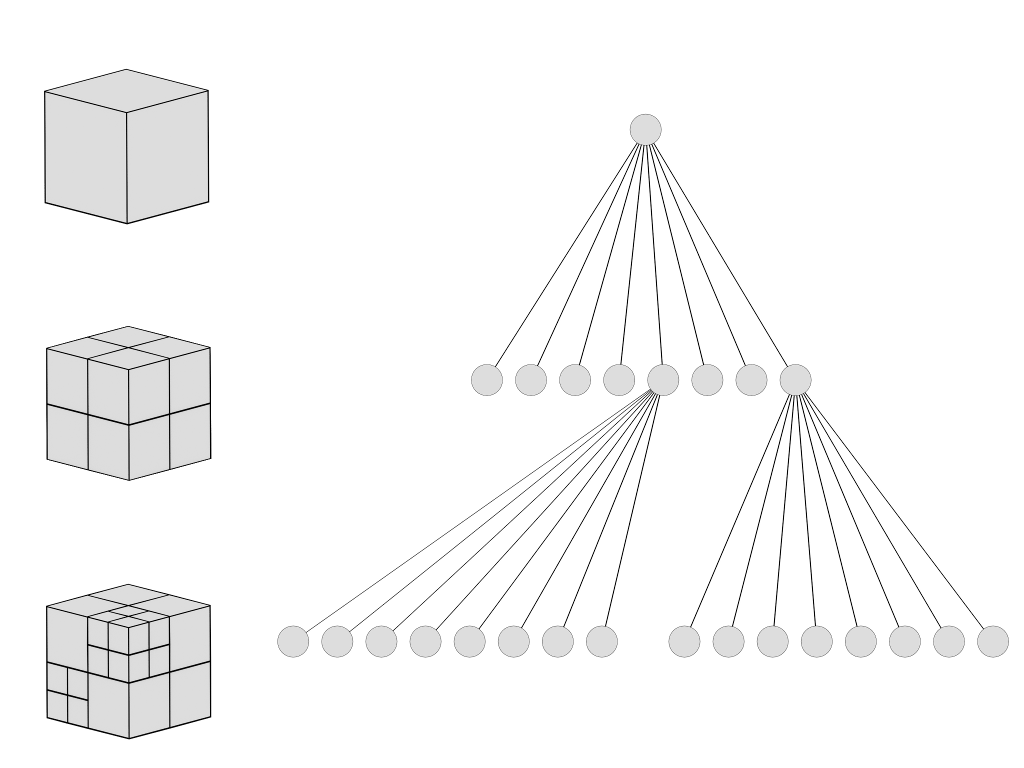
\includegraphics[width=0.95\textwidth]{ocTree_levels.png}
  \caption{depiction of a simple \texttt{ocTree}. Left: 3D view, step-wise representation of the splitting process (downwards from the top). right: final 2D representation of the tree's structure}\label{fig:ocTree_levels.png}
\end{figure}


\pagebreak
\subsection{User selection}
\label{sec:user_selection}

This section covers the elementary functions that handle the selection of vertices through user input. The two crucial functions explained in the subsequent subsections implement means to add vertices to an initially empty set of vertices and remove them later if desired. Selected vertices are be visually highlighted in the application and, at any time, the current set of selected vertices can be saved to an external text file.

	\subsubsection{\texttt{addVerticesToSelectionByCoordinates()}}
	\label{sec:addVerticesToSelectionByCoordinates()}
This private, recursive function adds vertices to a set of selected vertices by reference, based on three-dimensional coordinates and a search radius. The following parameters are required:
\begin{enumerate*}
	\item An input coordinate depicting the point in real space where a user is using the input device (a \texttt{glm::vec3} is used in this work),
	\item A \texttt{float} value describing the radius around thee input coordinate in which vertices are to be added to the selection, and
	\item A reference to the set of indexes of vertices (\texttt{std::set<size\_t>} is used in this work)
\end{enumerate*}.

An additional boolean flag determing whether, during the recursive search for the correct node, information is printed to the console or not, is passed with a default value of \texttt{false}. If set to \texttt{true}, it causes information to be displayed. The general course of events within this function proceeds as follows:
\begin{enumerate}
	\item Check if any of the given input point's coordinates are located outside of the bounds of the root of the \texttt{ocTree} indexing the 3D object. Throws exception if this is the case.
	\item Check if the current node is a leaf (i.e. has no child nodes). This terminates the recursive search and proceeds with finding vertices around the given input coordinates, as it is safe to assume that the correct node is found.
	\item Add all vertices within this node to the set of vertices to be checked.
	\item Determine if the radius around the query point crosses the bounds of this node in any direction. If so, add all vertices of the neighbouring node to the set of vertices to be checked.
	\item Iterate over the entire set of vertices to be checked to find which ones lie in radius around the query point and add those to the set of selected vertices.
	\item If this node is not a leaf node - steps 3, 4 and 5 are skipped in this case - determine the correct child node in which the query point is located and have that node recursively call \texttt{addVerticesToSelectionByCoordinates()}.
\end{enumerate}

Consider figure \ref{fig:a01_without_neighbours} for a clear depiction of the process. For the sake of a simplified, clear presentation, an orthographic top view which only considers axes x and y is shown here. Four of an implicitly shown parent node's eight subtree nodes are shown. The figure illustrates, from left to right, three vital steps towards finding vertices that lie within a search radius $r$ around an input query coordinate $P_q$. Throughout these steps, $P_q$ is depicted as an orange point, $r$ is shaded blue. Vertices within this radius compose the result of the query $V_{result}$ and get added to the set of currently selected vertices. Vertices which are considered to get checked if they lay within $r$, $V_{check}$, are highlighted blue, the ones where this is not the case are plain gray.

\begin{figure}[htb]
  \centering
  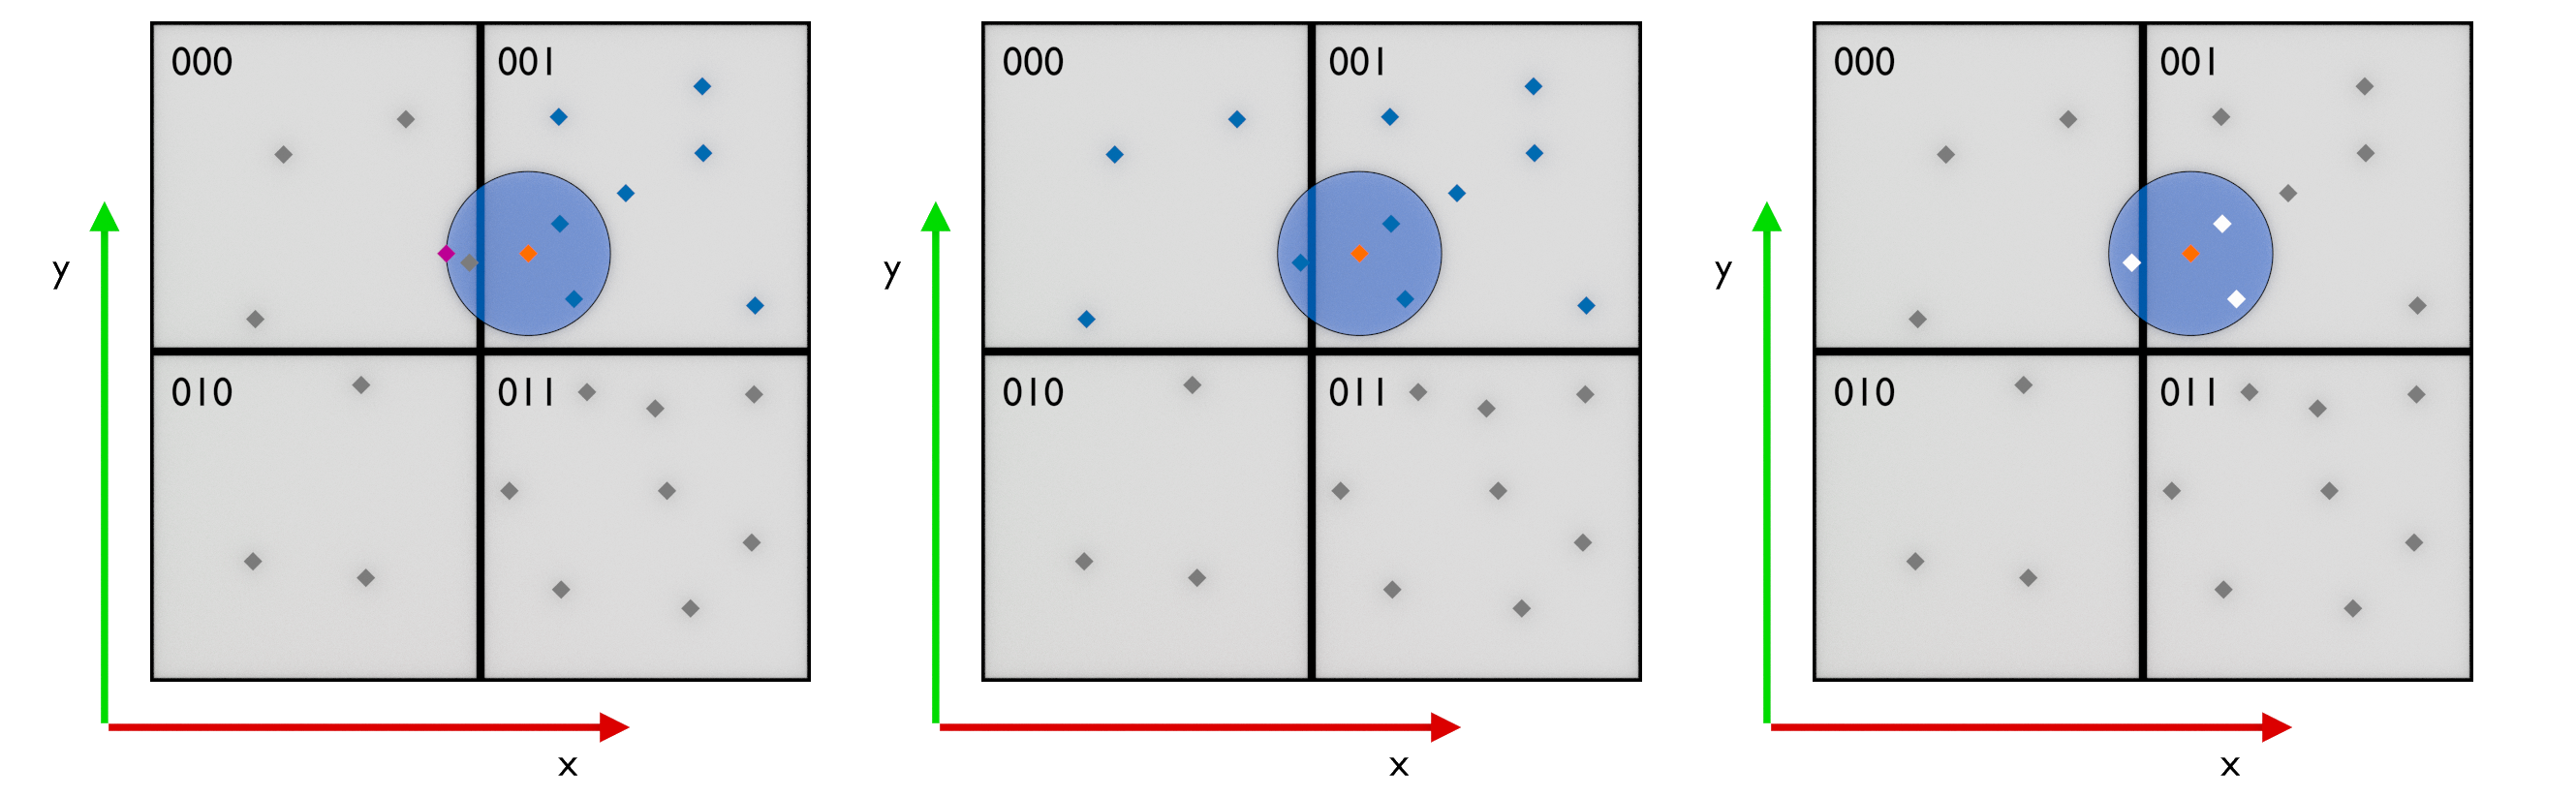
\includegraphics[width=1.0\textwidth]{a01_without_neighbors.png}
  \caption{Determing vertices to check and final set of selected vertices}\label{fig:a01_without_neighbours}
\end{figure}

The leftmost part of figure \ref{fig:a01_without_neighbours} shows the state after two crucial steps have already been taken: Leaf node $N_q$, i.e. the node that contains $P_q$ and does not have child nodes (001 in the figure) is found and all the vertices within it added to $V_{check}$ (highlighted blue). Furthermore, since the search radius around $P_q$ crosses the bounds of $N_q$ in negative x direction, an additional call to \texttt{addVerticesToSelectionByCoordinates()} with parameters $P_{q}^{'}$ and radius $r^{'}$ = 0 is executed, with $P_{q}^{'}$ = [$P_q.x-r$, $P_q.y$, $P_q.z$] (highlighted purple). This additional query found that $P_{q}^{'}$ is located in leaf node 000. Thus, as shown in the middle part of the figure, vertices in 000 are added to $V_{check}$. Note that one vertex that is located within $r$ - but not the bounds of $N_q$ is added to $V_{check}$ this way. The righthand part of the figure shows the result of the original query. After checking all vertices in $V_{check}$ whether they lie within $r$ around $P_q$, a set of vertices which fulfill this very condition $V_{result}$, containing three vertices (highlighted white) is returned.

The following code-snippets show how the process described above is implemented in this work.

\begin{minipage}{\linewidth}
\begin{lstlisting}[language=C++,numberstyle=\zebra{black!5}{white}{},numbers=left,xleftmargin=2em,tabsize=3]
ocTree* ocTree::addVerticesToSelectionByCoordinates(...) {
	if (target.x < m_minX || target.x > m_maxX || target.y < m_minY
		|| target.y > m_maxY || target.z < m_minZ || target.z > m_maxZ) {
		std::cout << "EXCEPTION" << std::endl;
		return NULL;
	}

	if (this->getisLeaf() == true) {
		result = this;
		std::vector<std::pair<size_t, glm::vec3> > verticesToCheck;
		for(size_t t = 0; t < result->m_verticesInBounds.size();++t){
			verticesToCheck.push_back(result->m_verticesInBounds[t]);
		}
		if (radius != 0) {
			glm::vec3 neighbourCo;
			if (target.x - radius < m_minX) {
				neighbourCo = {target.x-radius, target.y, target.z};
				ocTree * neighbour = m_root->addVerticesToSelectionByCoordinates
				(neighbourCo,0,intermediateSelection,debugInfo);
				verticesToCheck.insert
				(verticesToCheck.end(), neighbour->m_verticesInBounds.begin(),
				neighbour->m_verticesInBounds.end());
			}
			if (target.x + radius > m_maxX) {
				neighbourCo = {target.x+radius,target.y,target.z};
				ocTree * neighbour = m_root->addVerticesToSelectionByCoordinates
				(neighbourCo,0,intermediateSelection,debugInfo);
				verticesToCheck.insert
				(verticesToCheck.end(), neighbour->m_verticesInBounds.begin(),
				neighbour->m_verticesInBounds.end() );
			}
			// <repeat for y and z direction>
		}

		std::vector<std::pair<size_t, glm::vec3>>::const_iterator it;
		for (it = verticesToCheck.begin(); it!=verticesToCheck.end(); ++it) {
			if (radiusContainsCoordinates(r, it->second) {
				intermediateSelection.insert(it->first);
			}
		}
		return result;
	}
}
\end{lstlisting}
\end{minipage}

In lines 2 - 6, it is validated whether the input coordinates of $P_q$ given via \texttt{target} is located within the bounds of the calling node - that is usually going to be the root node of an \texttt{ocTree} structure. If this is not the case, \texttt{null} is returned.
If line 8 evaluates to \texttt{true}, this means that the current node is a leaf node and since given input coordinates do not lie outside its bounds, this has to be target node of the query $N_q$.

In line 10 - 13, a new \texttt{vector} of \texttt{pairs} consisting of \texttt{size\_t} values and \texttt{glm::vec3} vectors, representing the set of vertices to be checked is created. The \texttt{size\_t} parts of  \texttt{pairs} in this vector provide unique indexing, ensuring fast and direct access to each element. However, at this stage, this set only contains vertices within initial target node $N_q$. Without the rest of the code, vertices within one or multiple \textit{neighbour nodes} that contain $P_{q}^{'}$ vertices which sould get selected, would be ignored.

Line 14 - 36 show two out of six possible types of \textit{neighbour node queries} - both possible ways in which \textit{r} can cross the bounds of $N_q$ in x direction and how they are handled are illustrated. Note how parameter \texttt{radius} is used here (line 14). If it is set to 0, this request (which is also handled by \texttt{addVerticesToSelectionByCoordinates} can be classified as a \textit{neighbour query} which means that it cannot possibly envoke further \textit{neighbour queries}. In lines 17 and 28, varying intermediate versions of $P_{q}^{'}$ are derived by adding and subtracting \texttt{radius} to initial x value of $P_{q}$ after it is found that they are located within a neighbouring node of $N_q$ (lines 16 and 24). After this, assitional queries are processed via \texttt{addVerticesToSelectionByCoordinates} with crucial input parameters $P_{q}^{'}$ and \texttt{radius} = 0 (lines 18, 19 and 26, 27). Finally, the vertices within the found \textit{neighbour node} are added to the set of vertices to be checked (lines 20 - 22 and 28 - 30). As hinted by the comment in line 32, this process is repeated for y and z directions.

Before recursively returning the calling node in line 41, the most important part of this function - that is actually determining which vertices are located in raidus \textit{r} around input coordinates $N_q$ - takes place in lines 36 - 40. Here, we see a \texttt{for} loop through $V_{check}$, the set of vertices that lie within the bounds of $N_q$ as well as those within one or more \textit{neighbour nodes} $N_q^{'}$. The simple utility function \texttt{radiusContainsCoordinates} takes care of this. Note that, in case it evaluates to \texttt{true}, the \texttt{first} element of a pair within \texttt{verticesToCheck} (or $V_{check}$) is added to \texttt{intermediateSelection} (or $V_{result}$). This first element is a simple \texttt{size\_t} number which serves as a unique identifier for every vertex of the entire loaded object. This approach ensures that almost negligibly small amounts of data are actually transferred within the application - between server to client instances (see
\ref{sec:selection_process})
). Depending on what system architecture the application is ran on, these \texttt{size\_t} values only take 32 or 64 bits of space in memory, whereas \texttt{glm::vec3} take up to 12 times as much space.

Note that the code-snippet above only considers cases in which \texttt{radius} $r$ around $N_q$ crosses one set of bounds of \texttt{ocTree} nodes. However, it is a trivial observation of the conceptual structure of octrees that, depending on combinations of a large \texttt{radius}, a low maximum allowed number of vertices per node and a high maximum allowed \texttt{level}, critical situations could emerge. Such a situation could take place in a fine-grained octree structure with a large number of high level leaf nodes. For any node $N$ on a level $l$, the following is true.

$N_s$($d$) = $N_{R}$($d$) / $2^{l}$ where $N_s$($d$) is the size of $N$ in dimension $d$ and $N_{R}$($d$) is the size of root node $N_{R}$ in dimension $d$.

So in this application, after the object is loaded and spatially indexed, we consider the maximum allowed level for leaf nodes $l_{max}$ as well as the bounding values of its root node. The minimum difference between the maximum and mininum values in a dimension indicate the shortest dimension $d_{min}$ of the root node. Based on these values, we can set a maximum allowed value $r_{max}$ for the search radius as follows.

$r_{max}$ = $d_{min}$ / $2^{l_{max}}$ * 0.95. In other words, the maximum allowed search radius is 95\% the size of the smallest possible leaf node. Thus, no search query can evoke more than three additional queries for \textit{neighbour nodes}, one in each dimension.

Finally, the following simplified code-snippet shows how, making use of recursion, child nodes perform further calls to \texttt{addVerticesToSelectionByCoordinates} until $N_q$ (or $N_{q}^{'}$) is found, based on the directions in which $P_{q}^{'}$ crosses the bounds of the calling node.

\begin{minipage}{\linewidth}
\begin{lstlisting}[language=C++,numberstyle=\zebra{black!5}{white}{},numbers=left,xleftmargin=2em,tabsize=3]
ocTree* ocTree::addVerticesToSelectionByCoordinates(...) {
	// <cont.>
	if (target.x < m_meanX) {
		if (target.y < m_meanY) {
			if (target.z < m_meanZ) {
				// 110
				result = m_myChildren[6]->addVerticesToSelectionByCoordinates();
			} else {
				// 010
				result = m_myChildren[6]->addVerticesToSelectionByCoordinates();
			}
		} else {
			if (target.z < m_meanZ) {
				// 100
				result = m_myChildren[6]->addVerticesToSelectionByCoordinates();
			} else {
				// 000
				result = m_myChildren[6]->addVerticesToSelectionByCoordinates();
			}
		}
	} else {
		if (target.y < m_meanY) {
			if (target.z < m_meanZ) {
				// 111
				result = m_myChildren[6]->addVerticesToSelectionByCoordinates();
			} else {
				// 011
				result = m_myChildren[6]->addVerticesToSelectionByCoordinates();
			}
		} else {
			if (target.z < m_meanZ) {
				// 101
				result = m_myChildren[6]->addVerticesToSelectionByCoordinates();
			} else {
				// 001
				result = m_myChildren[6]->addVerticesToSelectionByCoordinates();
			}
		}
	}
}
\end{lstlisting}
\end{minipage}

Finding which child node $N_{l+1}$ is to perform the next recursive call happens in three simple \texttt{if - else} statements, the first one consisting of blocks of lines 3 - 20 and 21 - 39. In case the first \texttt{if} in line 3 evaluates to \texttt{true}, $P_q$ lies between the calling subtree node's minimum and mean values in x direction, thus the relevant child node's identifier must be \texttt{false} (0) at its \textit{level offset} $O_{l+1}$+2. If the statement in line 4 is \texttt{true}, the second $O_{l+1}$+1 can only be \texttt{true} (1). Whether the last value at $O_{l+1}$ is \texttt{true} or \texttt{false} is determined in line 5. We see exemplary, shortened recursive calls to \texttt{addVerticesToSelectionByCoordinates} in lines 7, 10, 13, 15, 18 and so on which are returned at the end of the function.

	\subsubsection{\texttt{removeVerticesFromSelectionByCoordinates()}}
	\label{sec:removeVerticesFromSelectionByCoordinates()}

This is the counterpart to \texttt{addVerticesToSelectionByCoordinates} and the second of two elementary methods that allow users to create and modifiy vertex selections in this application. Using the exact same parameters in identical order, it is a private, recursive function that allows for vertices added to the current selection to be removed again. In fact, the two functions vary so little, we can use the same list of general tasks as shown in \ref{sec:removeVerticesFromSelectionByCoordinates()}. The crucial differences are highlighted in bold text.

\begin{enumerate}
	\item check if any of the given input point's coordinates are located outside of the bounds of the root of the \texttt{ocTree} indexing the 3D object. Throws exception if this is the case.
	\item check if the current node is a leaf (i.e. has no child nodes). This terminates the recursive search and proceeds with finding vertices around the given input coordinates, as it is save to assume that the correct node is found.
	\item add all vertices within this node to the set of vertices to be checked.
	\item determine if the radius around the query point crosses the bounds of this node in any direction. If so, add all the vertices of the neighbouring node to the set of vertices to be checked.
	\item iterate over the entire set of vertices to be checked to find which ones lie in radius around the query point and \textbf{remove those from} the set of selected vertices.
	\item if this node is not a leaf node - steps 3, 4 and 5 were skipped in this case - determine the correct child node in which the query point is located and have that node recursively call \textbf{\texttt{removeVerticesFromSelectionByCoordinates()}}.
\end{enumerate}

At this point it is worth noting that these two fundamental functions were mapped to two different buttons on the hand-held controller used at the V2C. Figure \ref{fig:selection.png} shows a simple 3D object at various stages during consecutively performing these fundamental operations on it. The leftmost part of the figure shows a simple sphere with no vertices selected. The middle part shows the same sphere after eight vertices have been added to the selection and how they are highlighted. The righthand part of the figure shows the object after four vertices have been removed from the selection via \texttt{addVerticesToSelectionByCoordinates} with other coordinates.

\begin{figure}[htb]
  \centering
  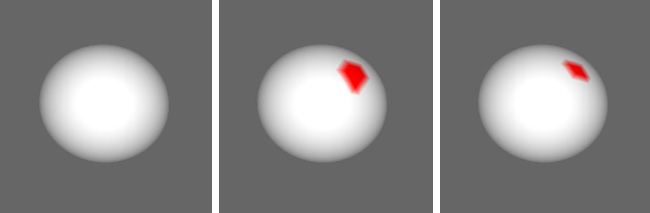
\includegraphics[width=0.9\textwidth]{selection.png}
  \caption{A basic vertex selection process}\label{fig:selection.png}
\end{figure}


\subsection{Tracking selection}
\label{sec:tracking_selection}

The set of user selected vertices is being kept track of as described in this section. Using the two fundamental functions described in \ref{sec:removeVerticesFromSelectionByCoordinates()} and \ref{sec:addVerticesToSelectionByCoordinates()}, every vertex of a spatially indexed 3D object can be selected and deselected at will. At each frame, every currently selected vertex is highlighted in an easily distinguishable bright red shade. Additionally, at any point during runtime, the server program of the application can print the current set of selected vertices to an external textfile.

Vertices in this application can either be selected or not selected. Only selected vertices are tracked. This is implemented using the following two variables in the main class.

\begin{description}
	\item[\texttt{std::set<size\_t> vertexSelection}] - a set of unsigned integers. A \texttt{set} is a C++ specific type of container with two handy properties for this use case. It guarantees the uniqueness of each element, as the value of an element is also the key used to identify it, and it is allocator-aware, which means it uses an allocator object to dynamically handle its storage needs (see \cite{set}).
	\item[\texttt{std::vector <std::pair <size\_t, glm::vec3> >  verticesList}] - A \texttt{vector} containing \texttt{pairs} of unique \texttt{size\_t} values and \texttt{glm::vec3} objects. \texttt{vectors} are contiguous storage containers that can store any type of objects, provide access to elements by using offsets (just like arrays) but also change their size dynamically (see \cite{vector}). Since the actual content of this variable is created and stored during spatially indexing a loaded 3D object during the recursive building process of an octree structure (see \ref{sec:buildTreeRecursively}), its final required size is not know at startup of the application, hence an ordinary \texttt{array} is not a suitable datatype here.
\end{description}

After the setup process of the application, \texttt{verticesList} essentially holds an ordered list of pairs of integer numbers and three-dimensional coordinates. Table \ref{tab:verticesList-startup} illustrates an excerpt of its possible content after startup. Note that the order of coordinates is arbitrary and, in no way, represents the structure or order of the loaded 3D file.

\begin{table}[]
\centering
	\begin{tabular}{l|l}
	offset (\texttt{size\_t}) & coordinate (\texttt{glm::vec3}) \\ \hline
	0 & [0.481, 0.461, 0.458] \\
	1 & [0.351, 0.335, 0.024] \\
	2 & [0.385, 0.324, 0.021] \\
	3 & [0.452, 0.342, 0.125]
	\end{tabular}
	\caption{content of \texttt{verticesList} at startup}
	\label{tab:verticesList-startup}
\end{table}
% table 4.3

\subsection{Synchronisation at the V2C}
\label{synchronisation_at_the_v2c}

The \textit{selection application} operates as a multi-threaded, synchronised program at the V2C. There is one server thread, performing operations on the octree structure, and multiple projection threads, keeping vertices that make up the projected object as well as their attributes up to date. The crucial set of data that must be synchronised for all threads of the program is the \texttt{std::set} object containing every currently selected vertex. To prevent this entire set to be exchanged in between threads at runtime, another temporary \texttt{set}, only storing newly selected vertices or those that are to be removed from the current selection.

In addition to input coordinates, the following two parameters are passed to calls to this function in the context of a user adding or removing vertices to the current selection: The pre-computed selection radius and a reference to a temporary set vertices, holding unique vertex IDs. After a query is terminated, the set of vertices found will be added to this temporary set. Due to the design of the synchronisation routine between server and client threads of this application, this set will be emptied before the result of each such query is returned and written to it. If the \textit{add} button is pressed, the content of the intermediate selection will be added to another set holding the list of currently selected vertices total. If the \textit{remove} button is pressed, each of the temporarily selected vertices is looked up in this second set and, in case it is found, removed from it. This approach prevents the total set of selected vertices to be sent from the server to all client threads at every frame during runtime. Only newly selected vertices (or those that are to be removed from the current selection) are sent across the application. The time for each action (in seconds since the application was started) is logged as well.

\subsection{Testing setup}
\label{sec:testing_setup}

This section describes the steps taken to ensure that the selection application meets all its requirements and ensures its key features described in section \ref{sec:key_features} are implemented correctly. While it is not formally verified that the application works correctly in every use case conceivable, it was tested up until a point where fluent, real-time and comfortable interaction was possible from a user perspective.

		\subsubsection{Test files}
		\label{sec:test_files}
While developing the selection application, 3D modeling software was used to create a set of simple test files that would be exported to .obj format so they could be used for testing purposes. These objects were designed to test whether common queries are handled quickly and correctly as well as what happens in unfortunate edge cases. Such a fairly complex edge case is depicted in figure \ref{fig:edge_case}.

\begin{figure}[htb]
  \centering
  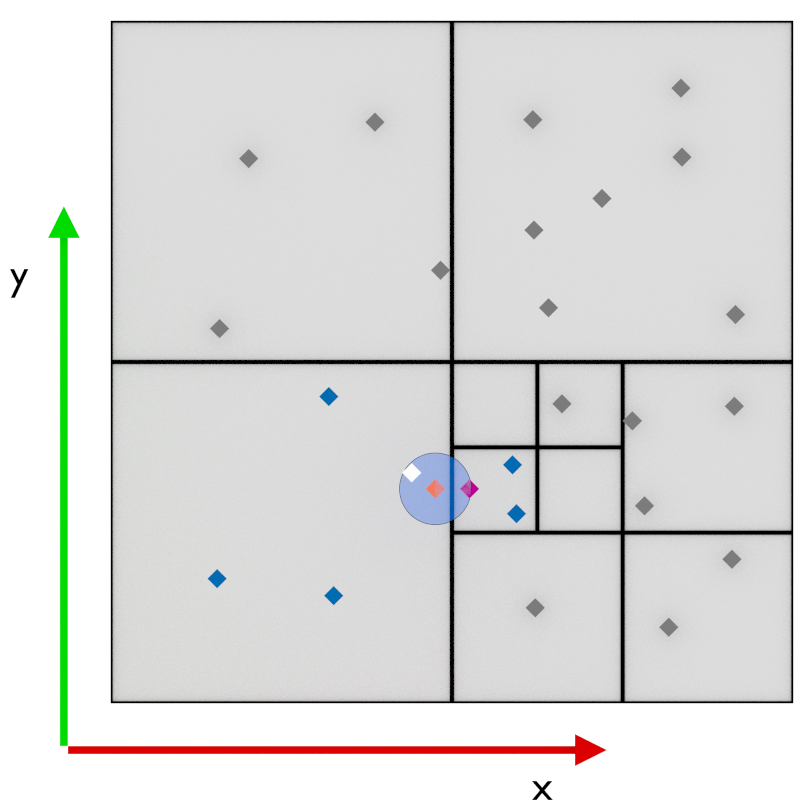
\includegraphics[width=0.5\textwidth]{edge_case.png}
  \caption{A fairly complex query to the octree structure of the selection application}\label{fig:edge_case}
\end{figure}

For the sake of readability, figure \ref{fig:edge_case} depicts an orthographic view on the structure of a test file used, showing only x and y axes. In such a case, all vertices shaded blue must be considered but only the one vertex shaded white is a correct result to the query. An additional query with input coordinates depicted by the point shaded in purple and radius 0 must be invoked and correctly handled as well, since the righthand border of the target node is crossed by the search radius. All vertices shaded gray must not be considered. The behavior of the application must be congruent to what is described in section \ref{sec:addVerticesToSelectionByCoordinates()}.

\begin{figure}[htb]
  \centering
  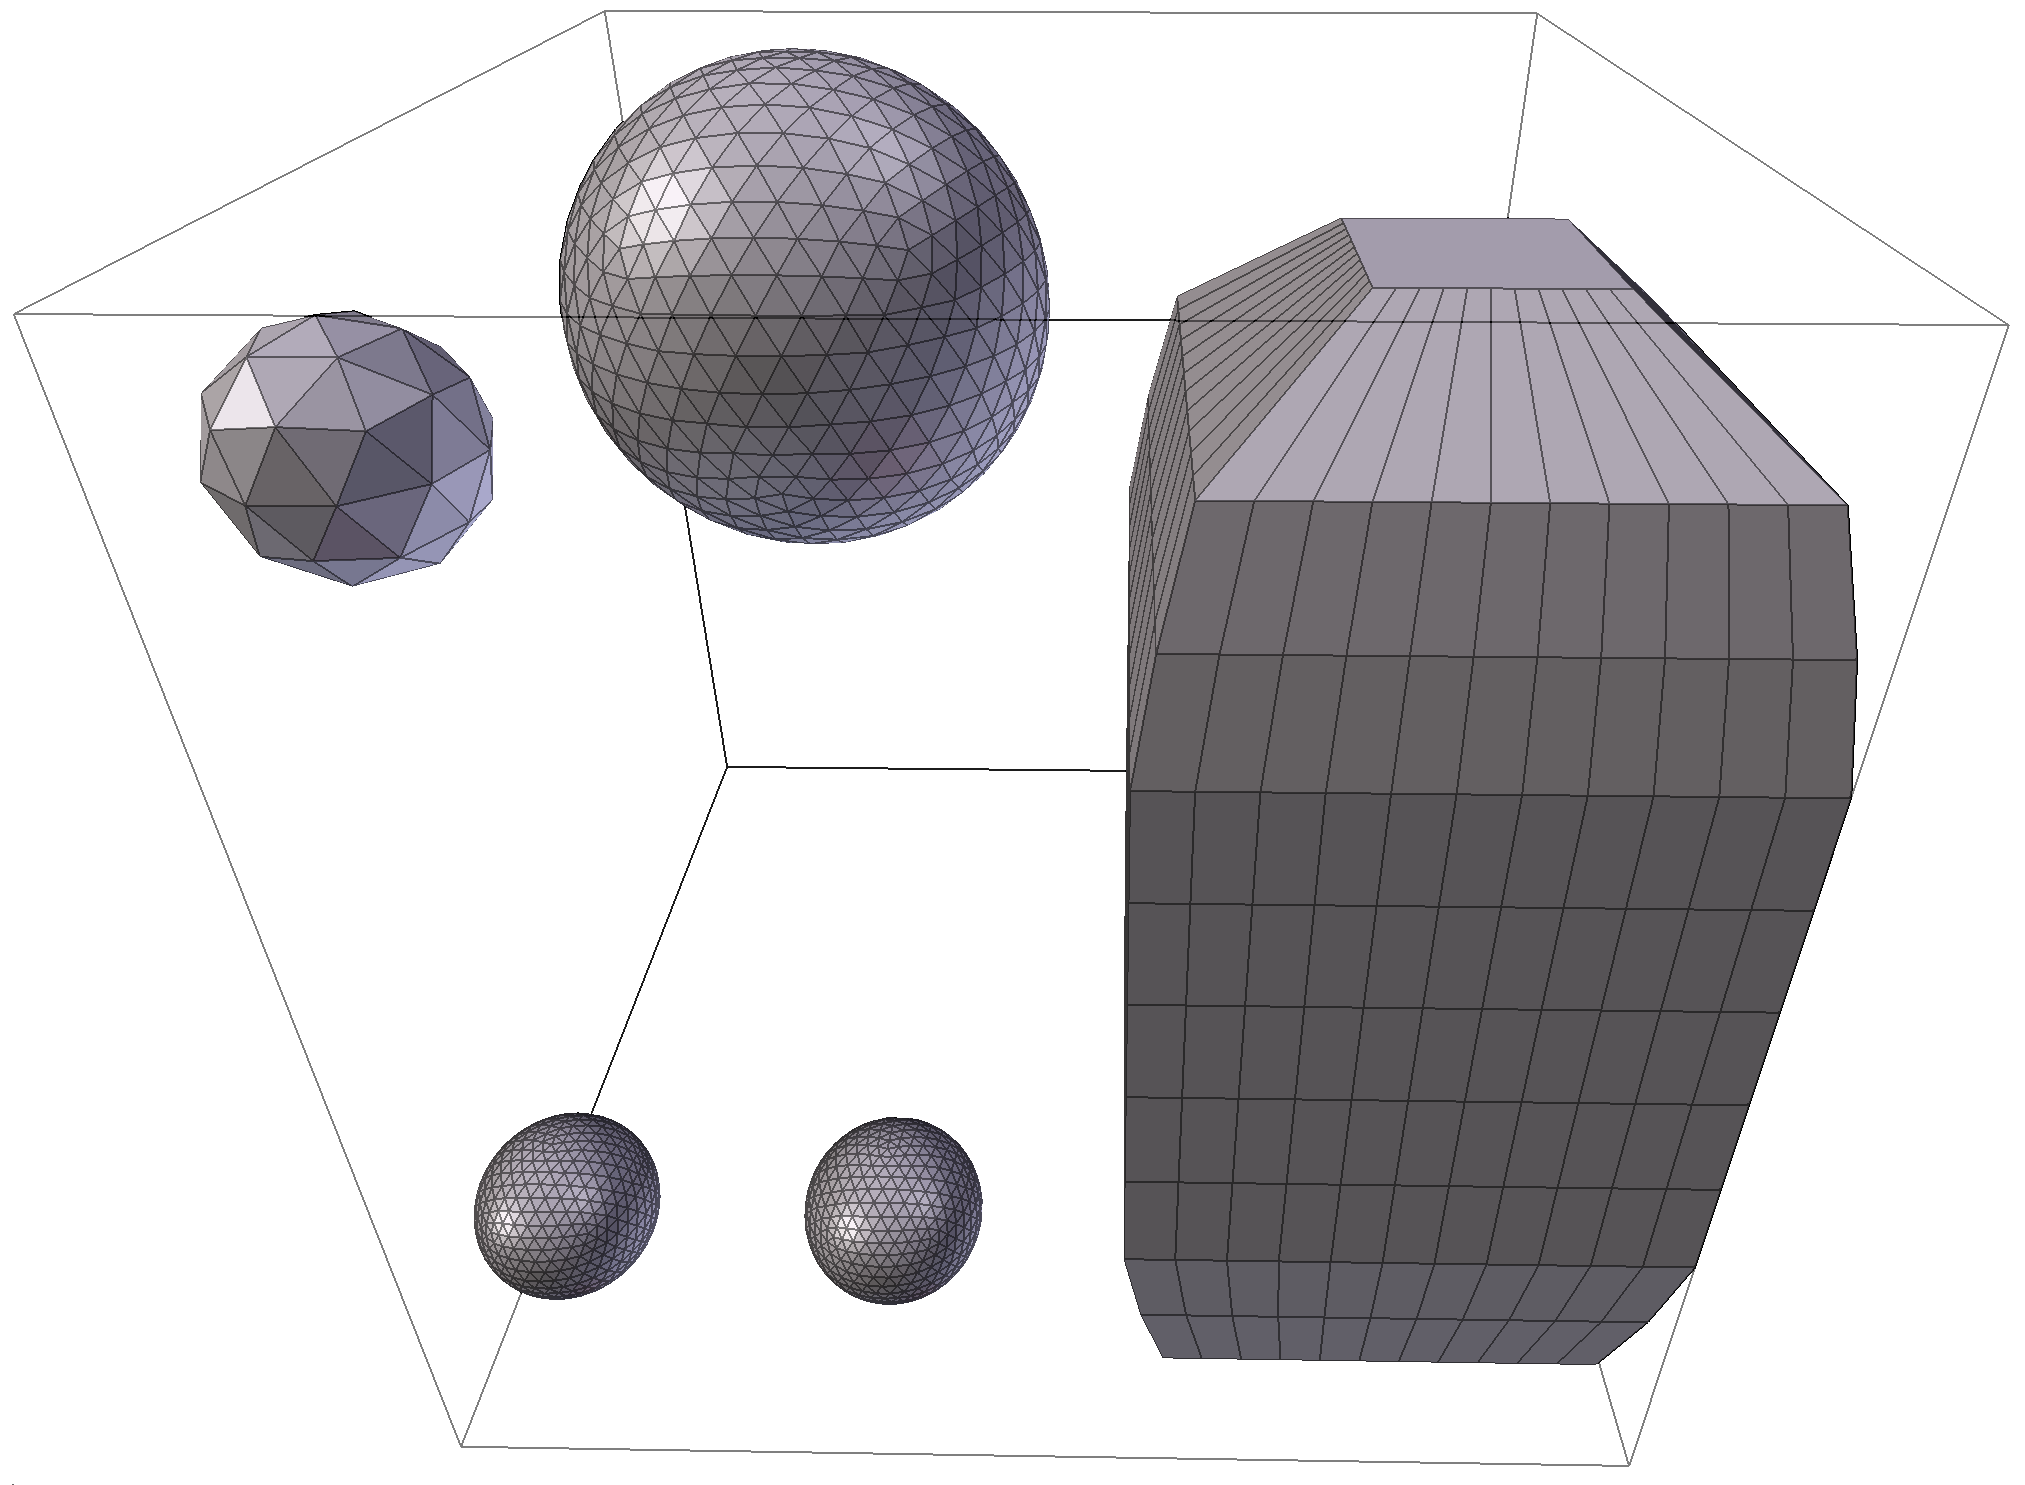
\includegraphics[width=0.75\textwidth]{test_file.png}
  \caption{A test file used during implementation, perspective view. Its bounding box and edges are depicted}\label{fig:test_thing}
\end{figure}

Figure \ref{fig:test_thing} shows a test file used during all stages of implementing the selection application. It is designed for the octree structure to be built in a clearly predictable way. For each combination of the maximum allowed number of vertices per node and the maximum allowed level, construction of the structure can be precisely predicted because all parts of the object are positioned in eighths of the space encapsulated by its bounding box. This file was used to a great extent for many testing queries as well as debugging.

The debugging process encompassed a multitude of test calls to the applications core functions using arbitrary coordinates as well as extensive use of the helper and debugging functions described in the subsequent subsection.

		\subsubsection{Helper and debugging functions}
		\label{sec:helper_and_debugging_functions}
The following functions which are non-essential to the functionality of the application are included. They were used during implementation for documentation, debugging and controlling the correctness of the core features. Parameters for these functions are omitted.

\begin{description}
	\item[\texttt{ocTree* getNodeByIdentifierArray()}] - gets a leaf node via a boolean input array representing its identifier. Traverses through an entire tree and returns the node with given identifier at the lowest level. The input boolean array has to contain $3*$ the maximum allowed split depth boolean values representing the identifier of a node. For example, at a maximum allowed split depth of 3, \texttt{false, false, false, true, true, false, false, true, true} is interpreted as 000110011 and a pointer to the according leaf node is returned.
	\item[\texttt{bool getIsLeaf()}] - determines whether this is a leaf or not. Returns private bool variable \texttt{m\_isLeaf}.
	\item[\texttt{void debugTreeInfo()}] - prints information about the finished \texttt{ocTree} object to the console, including total number of vertices stored by it, maximum allowed number of vertices per leaf, maximum allowed split depth and dimensions in x, y and z direction.
	\item[\texttt{void debugFirstVertex()}] - prints the coordinates of vertex at index 0 of \texttt{m\_vertices} to the console. This is a quick way to verify that import via ASSIMP worked.
	\item[\texttt{debugAllVertices()}] - prints the coordinates of all vertices to the console. This is a way to verify that import via ASSIMP worked correctly.
	\item[\texttt{void debugIdentifierasString()}] - prints the boolean identify array of the calling subtree to the console in an easily readable form, for example 001101.  Additionally, \texttt{m\_level} as well as the identifier array of the parent node of the calling subtree node are printed. If the calling node is the root, "I am root" is printed instead.
\end{description}

In addition, all essential functions of the \texttt{ocTree} class have an optional boolean parameter \texttt{debugInfo}, which is set to \texttt{false} by default. If set to \texttt{true}, information is printed to the console during execution of the functions. Depending on what function is called, this information varies strongly obviously. In general, all subtree nodes that recursively call any relevant functions as a result of the initially called function, call \texttt{debugIdentifierasString()}.

		\subsubsection{Testing at the V2C}
		\label{sec:testing_at_the_v2c}

Lots of hours were in the projection installation, testing the application. By experiencing the application from a user perspective, I wanted to make sure the feedback is quick, clearly noticeable and easily understandable. I tried to find bugs and wrong behavior by using the hardware in ways that were not planned on. Formally describing the procedure does not make sense, so consider the following brief descriptions of things I tried and what insights I gathered from them.

\begin{description}
	\item[Finding limitations to the tracking setup] - The projection installation of the V2C is 2.7 meters in width, height and depth. I tried to find out where the tracking system was working reliably and precisely and where the tracked space ended. I did not take exact measures but I found out that at a distance of about 30 centimeters away from the walls and the floor, the tracking started to get inaccurate. The positions of the tracked devices would freeze at the last position it was tracked correctly, thus making further selection or deselection operations impossible as well as leading to wrong projection of the scene.
	\item[Finding limitations to response time] - At a slow pace of movements, the projection thrown onto the walls surrounding the user, the visual feedback on where selection operations take place as well as indication of their results are in perfect synchronisation with what a user would expect. However, when moving the hand-held input device rapidly, its tracked position would get corrupted and the bright green object indicating its position within the 3D scene would only be rendered every dozen or so frames, being frozen in place in the meantime.
	\item[Finding limitations to synchronisation] - During the testing phase and the user study, the application froze multiple times. One or more projection programs would not react anymore, leaving no option but force-quitting and restarting the application. I was not able to reproduce this behavior. I can only speculate, based on various times trying this myself, that if a button is pressed for an ongoing timespan while rapidly moving the hand-held input device, this behavior seemed to occur mor frequently. Again, a formal description of what happened as well as the reasons why it happened can not be provided. A more extended testing and bugfixing process would be needed and this goes beyond the scope of this work.
	\item[Evaluating immersion and projection quality] - As described in section \ref{sec:technical_issues}, the framerate of the projection onto the the top wall was noticeably higher than those of the other projectors. During the user study, no remarks regarding this were made but from a developer stance, this can potentially impair immersion. Upon taking a look as close as possible to details of projected objects, the overlay of the two projections became visible, causing an incorrect spatial effect and blurriness. However, this only was noticeable when the tracked stereoscopic glasses got really close to the surface of a projected model.
\end{description}

In conclusion, it is fair to say that the \textit{selection application} provides clear feedback on what is happening based on user interaction and interaction is possible at a not too fast movement speed. Users should keep in mind that the tracking system has limitations. Not getting close to walls and not moving the hand-held input device rapidly while simultaneously keeping buttons pressed ensures a convenient, fluent interaction.


	\chapter{User study}
\label{sec:user_study_chapter}
%
% USER STUDY CHAPTER
%

From August 21th to September 12th 2017, a user studythat aimed at gathering data to compare with the results of processing 3D objects according to \textit{mesh saliency} \cite{lee2005mesh} was conducted. However, due to the fact that the projection installation at the V2C was not available at all times, it did not last for every single day of that timespan. The installation was assigned to this work for a total seven days. A reasonable amount of data from a sufficiently sized group of participants was collected. This chapter contains details on how the user studay was planned and conducted.

As briefly described before in section \ref{sec:conduct_user_study_with_the_selection_application}, participants were asked to use the \textit{selection application} and the hardware available at the V2C to select regions of 3D objects they found \textit{interesting}. In general, participants got familiar with the devices and interaction mechanics quickly and were able to make selections according to their perception of what was of importance. The resulting ratios of overall differences between \textit{mesh saliency} and \textit{user saliency} are fairly low for the three objects used in this work, ranging from about 0.23 to 0.38. However, whether this can be used as basis for any type of statement regarding how differently important parts of 3D data are recognised by humans in VR and computational, automatic procedures, is doubtful as discussed at the end of this chapter.

	\section{Hardware used}
	\label{sec:hardware_used}
%
% HARDWARE USED
%

The five-sided projection installation at the V2C is equipped with several devices which can be tracked inside of it. Users taking part in the user study were asked to put on a pair of lightweight stereoscopic glasses, shown in figure \ref{fig:concept_hardware}. Note the three white, spherical parts on each side of the glasses. These are used for tracking their position, orientation, tilt and yaw within the projection installation. According to these parameters, two images are projected onto the walls of the installation from behind, each for one eye. The glasses are in synchronisation with the projectors and actively switch between left and right 120 times per second, only showing one of the projected images at a time. This way, an immersive 3D effect for one user wearing the glasses within the installation is created.  

For interaction, a hand-held device called \textit{wand} see figure \ref{fig:concept_hardware}, is used within the projection installation. It allows for navigation within the scene via a little joystick as well as interaction with four buttons. The joystick moves the scene in the opposite way the user pushes it. This has been described as counter-intuitive by some users.

As described in section \ref{sec:selection_process}, two of the three buttons surrounding the joystick are enough for the selection application's needs. The two essential functions of the application are mapped to them in the following way. The button on top of the \textit{wand}, on the left side of the joystick is used for making selections on the currently loaded 3D object, the button  right to it can be used to clear already marked selections. Figure \ref{fig:concept_hardware} shows the device. Again, note the white, spherical parts used for tracking position, orientation, tilt and yaw of the device attached to it.

\begin{figure}[htb]
  \centering
  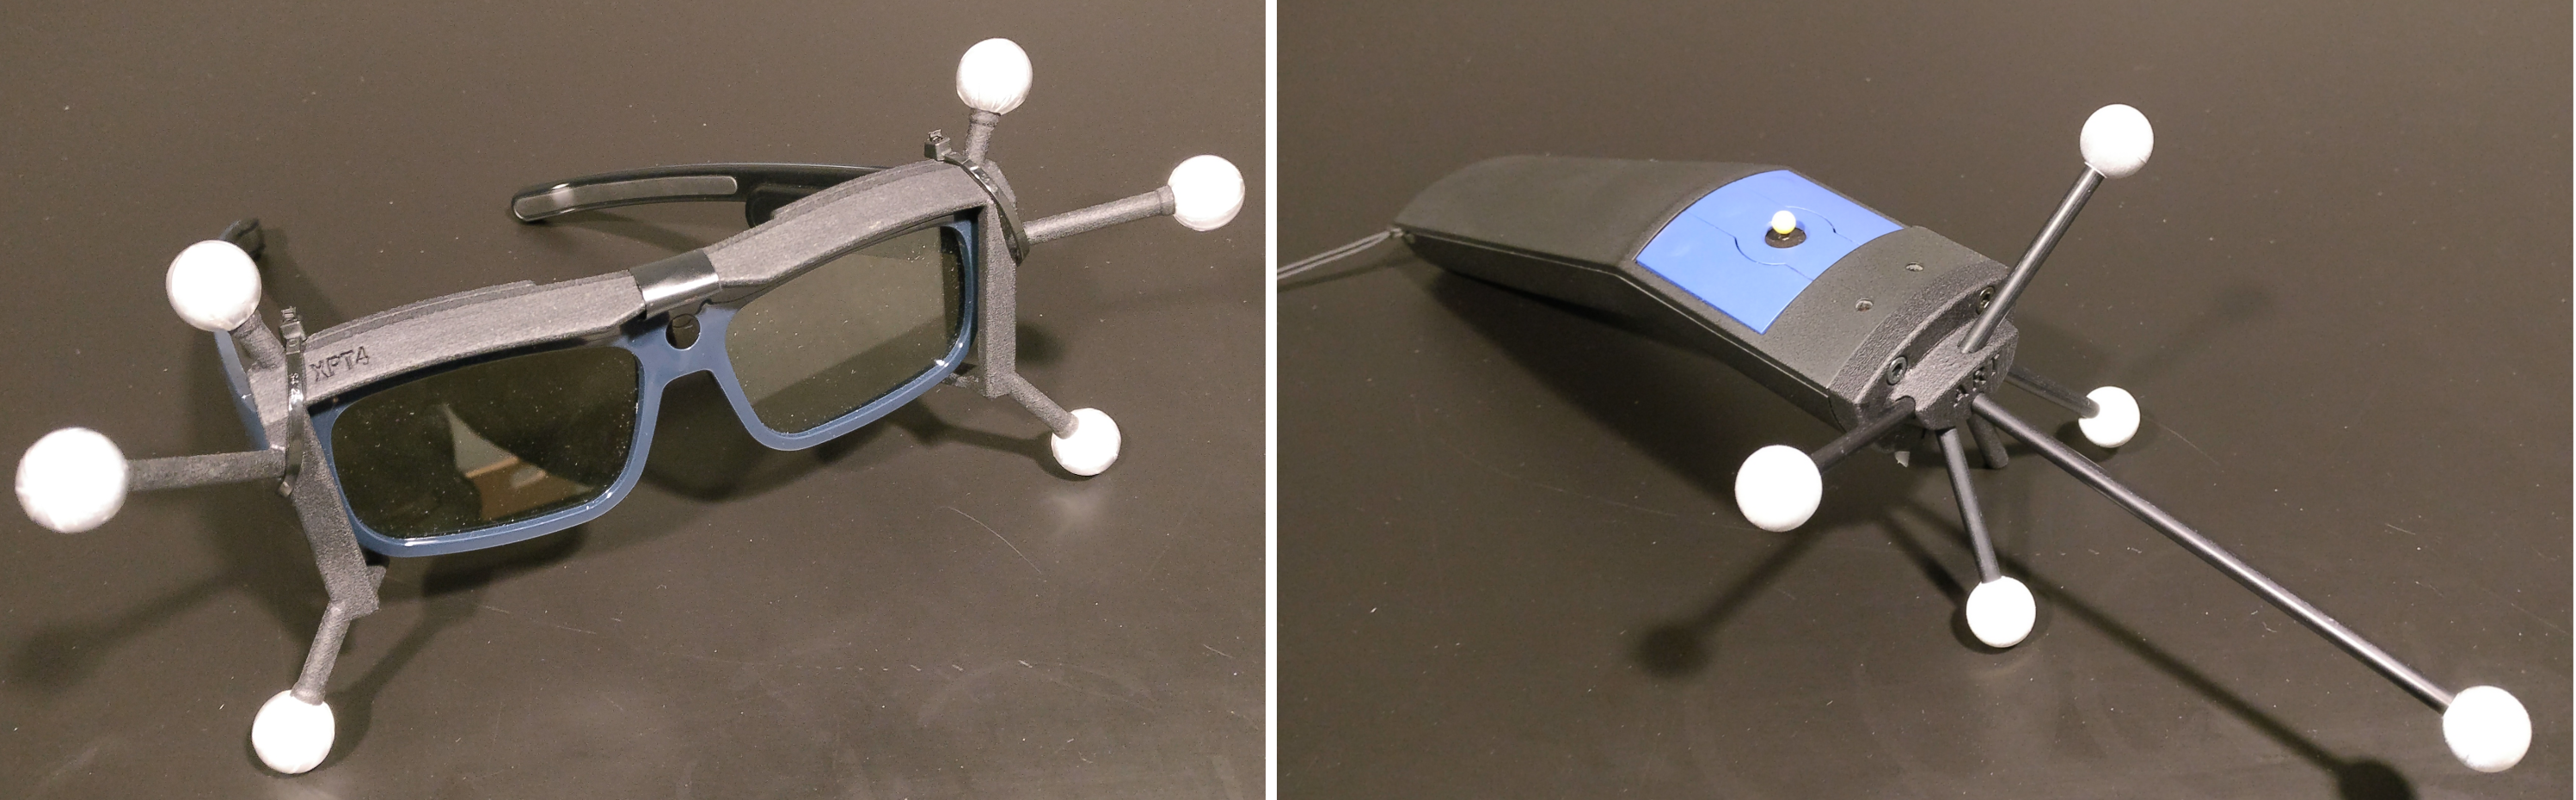
\includegraphics[width=.95\textwidth]{concept_hardware.png}\\ % PNG-File
  \caption{The hardware components available at the V2C. Left: A pair of active, stereoscopic shutter glasses. Right: The main input device, referred to as \textit{wand}}
  \label{fig:concept_hardware}
\end{figure}

\begin{figure}[htb]
  \centering
  \includegraphics[width=.8\textwidth]{selection_cave.png}\\ % PNG-File
  \caption{The selection process using the available hardware at the V2C}\label{fig:selection_cave}
\end{figure}

Figure \ref{fig:selection_cave} depicts what the selection process inside the projection installation at the V2C is like form a user perspective. Users utilise the \textit{wand} for navigation as well as selecting and deselecting parts of the presented objects they deem \textit{interesting}. The stereoscopic glasses provide a spatially convincing, three-dimensional immersion of the object. In the figure, the object is a simple cube with two iterative subdivisions. Its vertices are shaded gray, the edges connecting them are shaded black. The diamond-shaped object indicating the position of the \textit{wand} within the 3D scene is shaded bright green. The blue circle around it represents the spherical query radius for selection and deselection operations. Vertices within that lie within that circle are shaded orange. Figure \ref{fig:real_selection} shows a real selection process within the projection installation at the V2C.

\begin{figure}[htb]
  \centering
  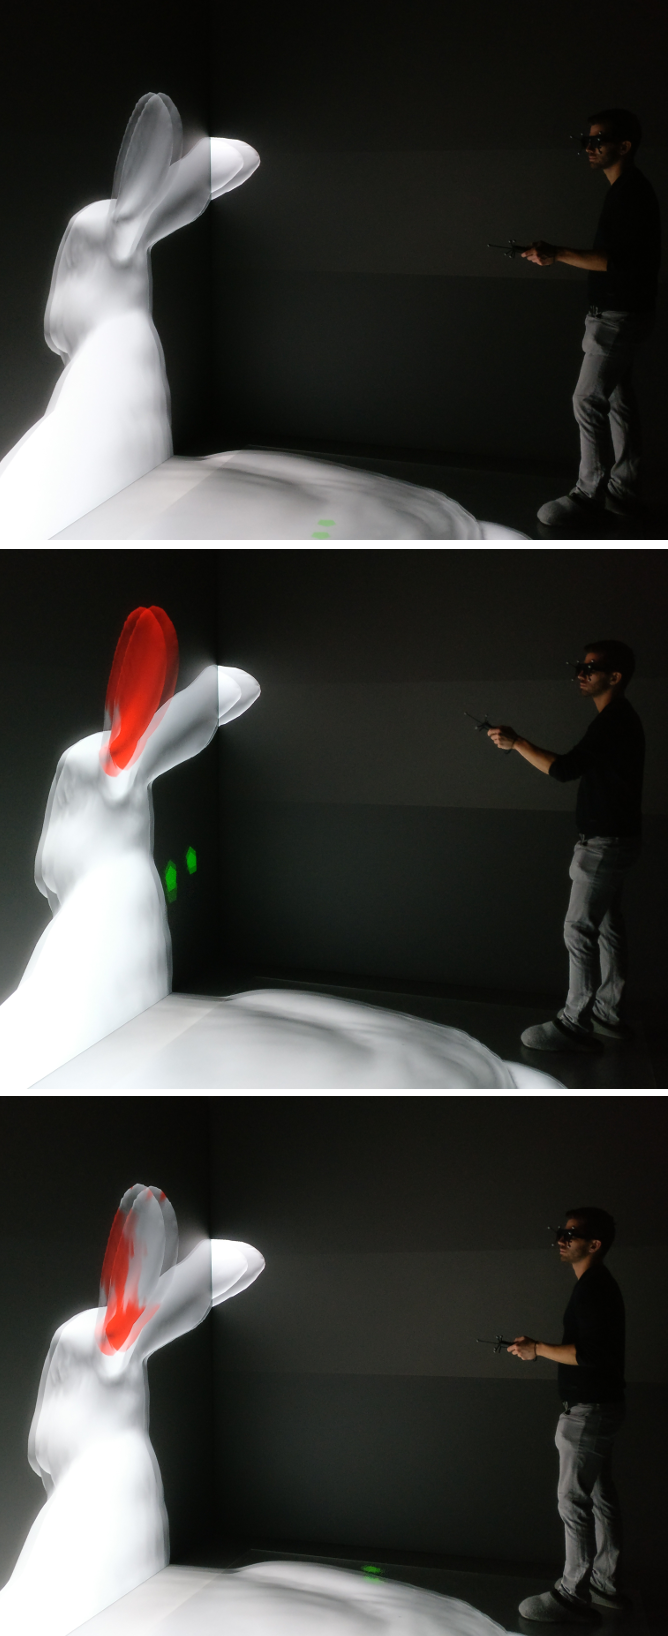
\includegraphics[width=0.6\textwidth]{real_selection_row.png}\\ % PNG-File
  \caption{A real selection process}\label{fig:real_selection}
\end{figure}

Consider figure \ref{fig:real_selection}. Starting with the top photograph of the figure, it shows a loaded, spatially indexed object where with nothing selected yet. The middle photograph shows the same object after a selection has been made. The bottom photograph shows the object after vertices have been deselected again. Note the green object that is also projected onto the walls. For the user, through the tracked glasses, it is visible at the tracked location of the input device at all times.

	\section{Models used}
	\label{sec:models_used}
%
% MODELS USED
%

\begin{figure}[htb]
  \centering
  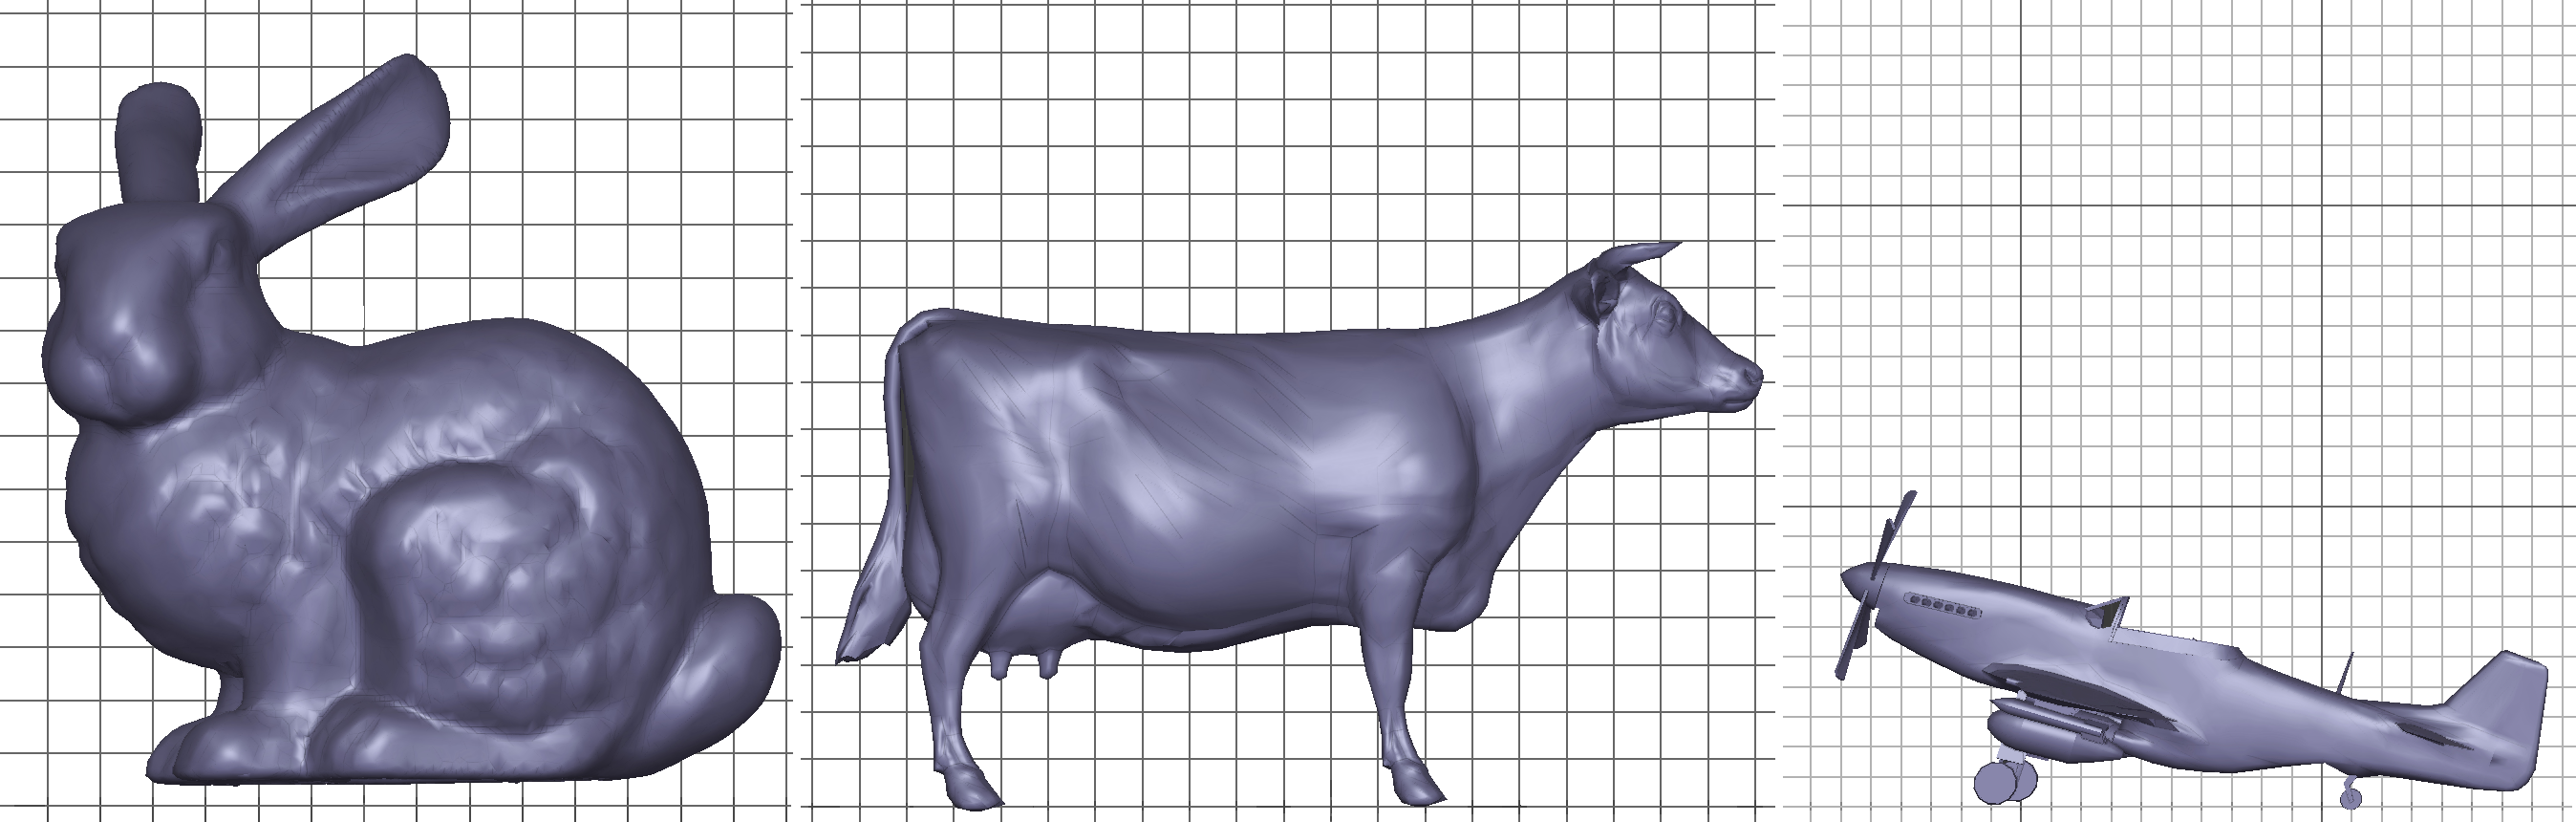
\includegraphics[width=1.0\textwidth]{userstudy_all_objects.png}\\ % PNG-File
  \caption{The 3D objects used for the user study}\label{fig:all_objects}
\end{figure}

Objects used for the study were chosen with the goal of offering as much variety of types of objects among as few objects as possible in mind. The motivation for this was to achieve results that are generally applicable for any type of geometric data, at least to an basic extent. Also, to avoid the users losing motivation due to repeating tasks during the study, keeping the number of objects to a minimum was a constraint to be considered. The three final objects chosen are described in table \ref{tab:userstudy_objects} and depicted in figure \ref{fig:all_objects}. Note that the models are from third-party vendors. I made sure they are all free to use for educational purposes and weblinks to where they have been published originally are provided in the bibliography.

Figure \ref{fig:all_objects} shows the objects used in the user study. From left to right, the 3D scanned bunny, the modelled cow and the low-poly, modelled aircraft are shown. Consider the grid to get a sense of their proportions. They were not scaled according to their real world sizes and instead made to take up approximately equal space in the virtual scene. This was done with the intention to provide a similar level of visual detail, independent of the actual geometric level of detail, for each object. Furthermore, the size of the objects was intended not to have any sort of influence on how users would perceive them.

\begin{table}[]
\centering
	\begin{tabular}{l|l|l|l|l}
		object	& created through	& source	& vertex count	& class of objects	\\ \hline
		cow	& 3D modelling		& \cite{cow}	& 69,648	& purely natural	\\
		P51 Mustang	&	3D modelling	& \cite{P51}	& 51,708	& purely mechanical	\\
		bunny sculpture	&	3D scan	& \cite{bun}	& 68,754	& natural, man-made	
	\end{tabular}
	\caption{3D objects used in the study}
	\label{tab:userstudy_objects}
\end{table}
% table 3.1

	\section{Tasks given}
	\label{sec:tasks_given}
%
% TASKS GIVEN
%

Users were asked to use the hard- and software available to select regions and parts of the objects they deemed \textit{interesting} since \textit{mesh saliency} claims to be able to reliably predict such parts \cite{lee2005mesh}. They were instructed that this would be the first real task at hand, after they stated they felt ready to interact with the scene presented in the projection installation. They were given as much time as they wanted to get somewhat accustomed to navigating and the selection process it but in general, nobody took longer than a few minutes.

Then, the course of the user study was explained and the following instructions were given.
\begin{itemize}
	\item The task is to select parts and regions of the objects users consider \textit{important}.
	\item Some suggestions as to what could be considered \textit{important}:
		\begin{itemize}
			\item \textit{what do you consider visually interesting or important?}
			\item \textit{what do you assume are natural focus points of attention?}
			\item \textit{what parts do you consider vital for identifying the object?}
		\end{itemize}
	\item However these are just ideas, in general users were encouraged to select whatever they, personally, deemed \textit{important} according to their own understanding. This was emphasised, aiming for \textit{natural} user selections.
	\item There is no \textit{correct} way to make the selection. Users were, again, encouraged to make selection according to their perception.
	\item How precise the selections would be was up to users. If they were satisfied, that was the desired level of precision
	\item I asked to consider symmetry to some extent in the selection where possible.
	\item The time limit per object was five minutes. It was made clear that the selection process would be stopped after that period of time.
	\item However, if users would be satisfied with the selection earlier, they were encouraged say so. In this case, if there were still objects left to work with, the next one would be presented. Otherwise, the practical part of the user study was finished.
\end{itemize}

	\section{Questionnaire}
	\label{sec:questionnaire}
After users completed the \textit{practical} part of the study, they were asked to fill out a short questionnaire, determined to acquire demographic data about the participants as well as feedback as to how they perceived interacting with the selection application. The data gathered through this is presented in section \ref{sec:participant_demographics}. 

The questionnaire was two pages total. It can be found in the appendix of this work. After stating that user data would be used anonymously and not be provided to any third parties, I also made sure to leave my contact information on the questionnaire. After this, the first page contained single-choice questions about gender, age, profession, prior experience with VR technology and whether the user was strongly visually impaired. Page two contained statements to which participants were asked to respond to in terms of how strongly they agree or disagree to with them. The (translated) statements read as follows:

\begin{itemize}
	\item \textit{I am interested in technology in general.}
	\item \textit{I am interested in VR/AR technology.}
	\item \textit{I easily got familiar with the selection application.}
	\item \textit{The spatial impression within the projection installation was convincing.}
	\item \textit{Navigating within the selection application felt comfortable and / or intuitive.}
	\item \textit{The selection process felt comfortable and / or intuitive}
	\item \textit{The selection process felt precise}
\end{itemize}

Users were asked to rate each of these statements on a Likert-scale. I offered five options to chose from:
\begin{enumerate*}
	\item \textit{I strongly disagree},
	\item \textit{I disagree},
	\item \textit{No comment},
	\item \textit{I agree} and
	\item \textit{I strongly agree}
\end{enumerate*}.
An example of the questionnaire (in German) can be found the appendix of this work.

	\section{Shortcomings of the study design}
	\label{sec:shortcomings_of_the_study_design}
While conducting the user study, some factors became noticeable that possibly had negative impacts on user behavior during the study and, consequently, its results. On top of that, a few technical issues emerged which could have made the experience for the users less immersive and convincing. The following subsections will briefly go over these issues. Whether they had any influence on the results of the study, or to what an extent is not described, the following is solely meant to document them.

		\subsection{Task, instructions and questions}
		\label{sec:task_instructions_questions}
While the tasks and questions (see section \ref{sec:questionnaire}) were designed to be as clear as possible, during conducting the user study, some flaws became prominent. For more on what users remarked, see section \ref{sec:individual_feedback_and_comments}. The following notes document my own, personal observations.

\begin{itemize}
	\item The task of selecting \textit{interesting} parts of the objects is both hard to describe and possibly not close enough to what \textit{mesh saliency} is meant to identify. What is \textit{interesting} and what is not, is a very personal, subjective decision, so results are bound to vary strongly. Participants in the user study were encouraged to select parts of the objects based on their personal perception and understanding of the term \textit{interesting} because a wide range of results was desired. However, a more uniform definition of terms might have been a reasonable basis for the comparison at the centre of this work too.
	\item As a result of the former note, adding an opportunity to rate the instructions given on the questionnaire might have given more insights as to how well designed the user study really was. After taking some time to get familiar with navigation within the projection installation and using the selection application, I made sure users had no questions left before the actual study was started. Questions here were very scarce so this note is not directly based on user feedback. However, as the study went along, I noticed that this could have been a valuable addition to the questionnaire.
	\item Another possibly relevant question I missed to put on the survey was whether users felt pressured by the time set time limit of five minutes per object. While the majority users proclaimed they were satisfied with their selection before time ran out, there were a few participants I had to stop after five minutes for every object. I chose the time limit to make sure users would not lose motivation over time and for the sole purpose of having a constant time factor. Again, I received no feedback from users indicating that this was an issue but explicitly asking them about it might have been relevant for completeness of this work.
	\item Regarding the rating of how much users agree or disagree to the statements on the second page of the survey, using \textit{I am indifferent} instead of \textit{No comment} as the third, neutral choice could have possible influenced the outcome of the study as well. I did not include this option on purpose because I explicitly wanted to avoid neutral answers while also not \textit{forcing} the users to make a decision.
\end{itemize}

		\subsection{Technical issues}
		\label{sec:technical_issues}
The projection installation at the V2C, while still fully functioning and performing well for the majority of time, is not the latest state-of-the-art anymore. The hardware has been in use for many years, some parts of it display signs of deterioration and some have even been replaced already. Maintenance work is frequently required. This section covers some aspects that were a result of this and may have had influence on user behavior during the study.

\begin{itemize}
	\item Weeks prior to the user study for this work started, parts of the projector that covered the top wall of the installation were replaced. This led to projections onto that wall running at a significantly higher frame rate. As a result, quick head movements, especially horizontal, with the image being spread over the upper wall and any of the others at the same time, caused the part visible on the upper wall to move much faster than the rest of the projection.
	\item On Monday, September 4th, the sixth day of the study, with five more days still ahead, one of the projectors died. The lower part of the \textit{southern} wall could not be used for displaying anything from then on. I had to advice users to try and only use the other sides of the installation but this certainly impaired the immersion. 
	\item Tracking of the stereoscopic glasses and the \textit{wand} did not work properly when they got near to the bottom or the walls of the projection installation. If they entered that \textit{outer area} of the room, projection would freeze in place until the user stepped closer to the centre of it again.
	\item This might have been a problem with my application - I could not reliably reproduce this error. Sometimes the application simply froze during the user selection process. I tried to reproduce this behavior but I can only speculate from what I have observed. This kind of freeze occurred more often when the \textit{wand} was moved very quickly over an extend period of time, while constantly pressing the \textit{select} button.
\end{itemize}


	\chapter{Results and discussion}
\label{sec:results_and_discussion}

\section{User study data}
\label{user_study_data}

\section{Individual feedback and comments}
\label{individual_feedback_and_comments}

\section{Interpretation}
\label{interpretation}

	\chapter{Conclusion and future work}
\label{sec:conclusion_and_future_work}

\section{Insights and conclusions}
\label{insights_and_conclusions}

\section{Future work}
\label{future_work}

    \vspace*{2cm}

   \textbf{I would like to thank...}


\vspace*{1cm}

My advisor Markus Wiedemann for his ongoing, patient and professional help during the course of this work. For helping me put things back in perspective whenever I felt overwhelmed by the workload in front of me and for making the most challenging aspects of this work seem less impossible to understand.


\vspace*{1cm}
His colleagues working at the Leibniz Supercomputing Centre, Thomas Odaker, Rainer Oesman and Dr. Rub\'{e}n Garcia Hern\'{a}ndez for letting me be a part of their dedicated, caring and inspiring working environment.


\vspace*{1cm}
My friend Christian Blank for helping me understand various concepts of software development. My friend Amy Eichorn for proof-reading and giving me a chance to practise writing in English. My friend Sebastian Dietl for inspirational discussions about theoretical aspects of this work.


\vspace*{1cm}
My friends Tobias Bjarsch, Christa Bichlmayer, Martin Erthel, Robert Hetzner and Manuel Miksche for their support and motivation throughout the duration of this work.


\vspace*{1cm}
The Ludwig Maximilian University of Munich, Prof. Dr. Dieter Kranzelm\"uller and the MNM-team for granting me the opportunity to conduct this work.


\vspace*{1cm}
My parents and family for their continuous and unconditional love and support.


% ---------------------------------------------------------------
\backmatter % ab hier keine Nummerierung mehr
    \listoffigures
    \bibliographystyle{alpha}
    \bibliography{./Bib/metz17}
    
\appendix

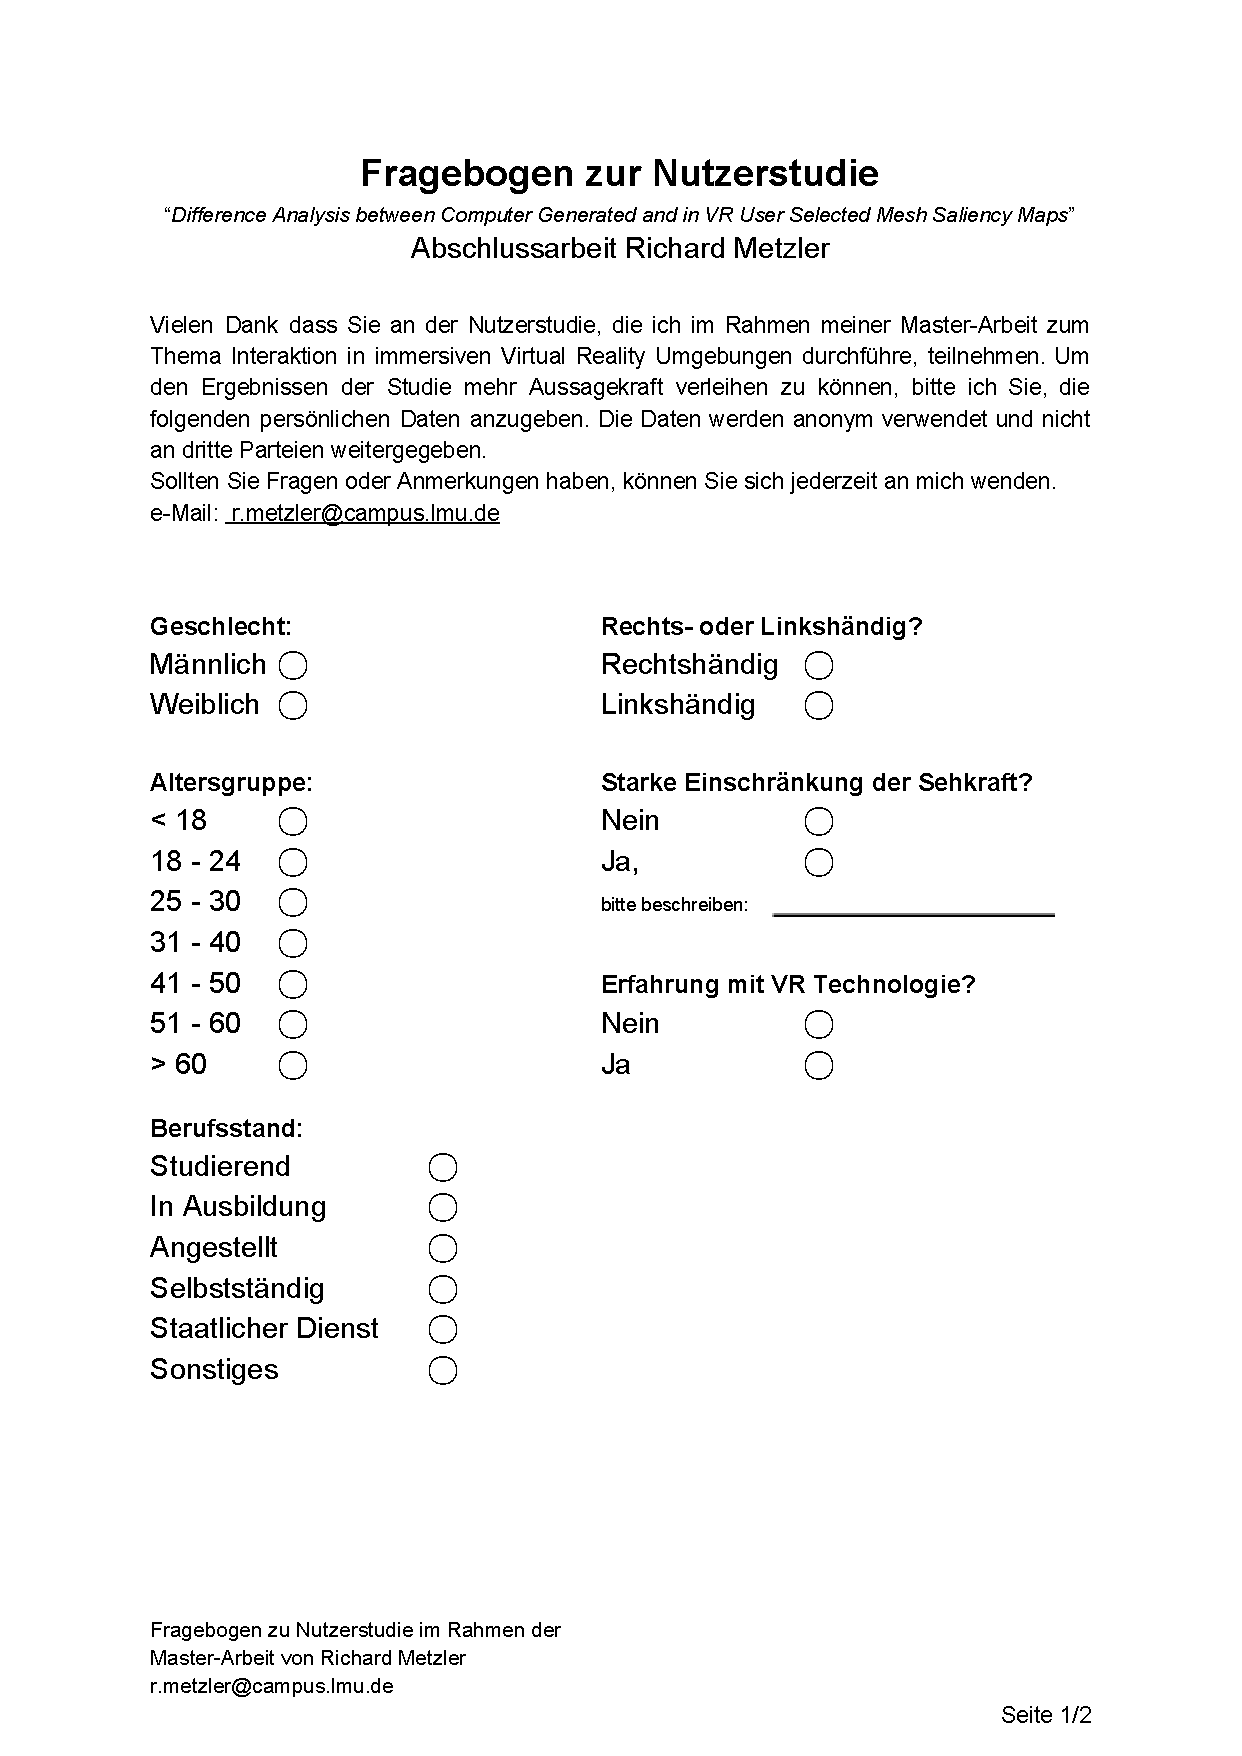
\includepdf[pages={1-2}]{appendix/Umfrage-08-26-2017.pdf}
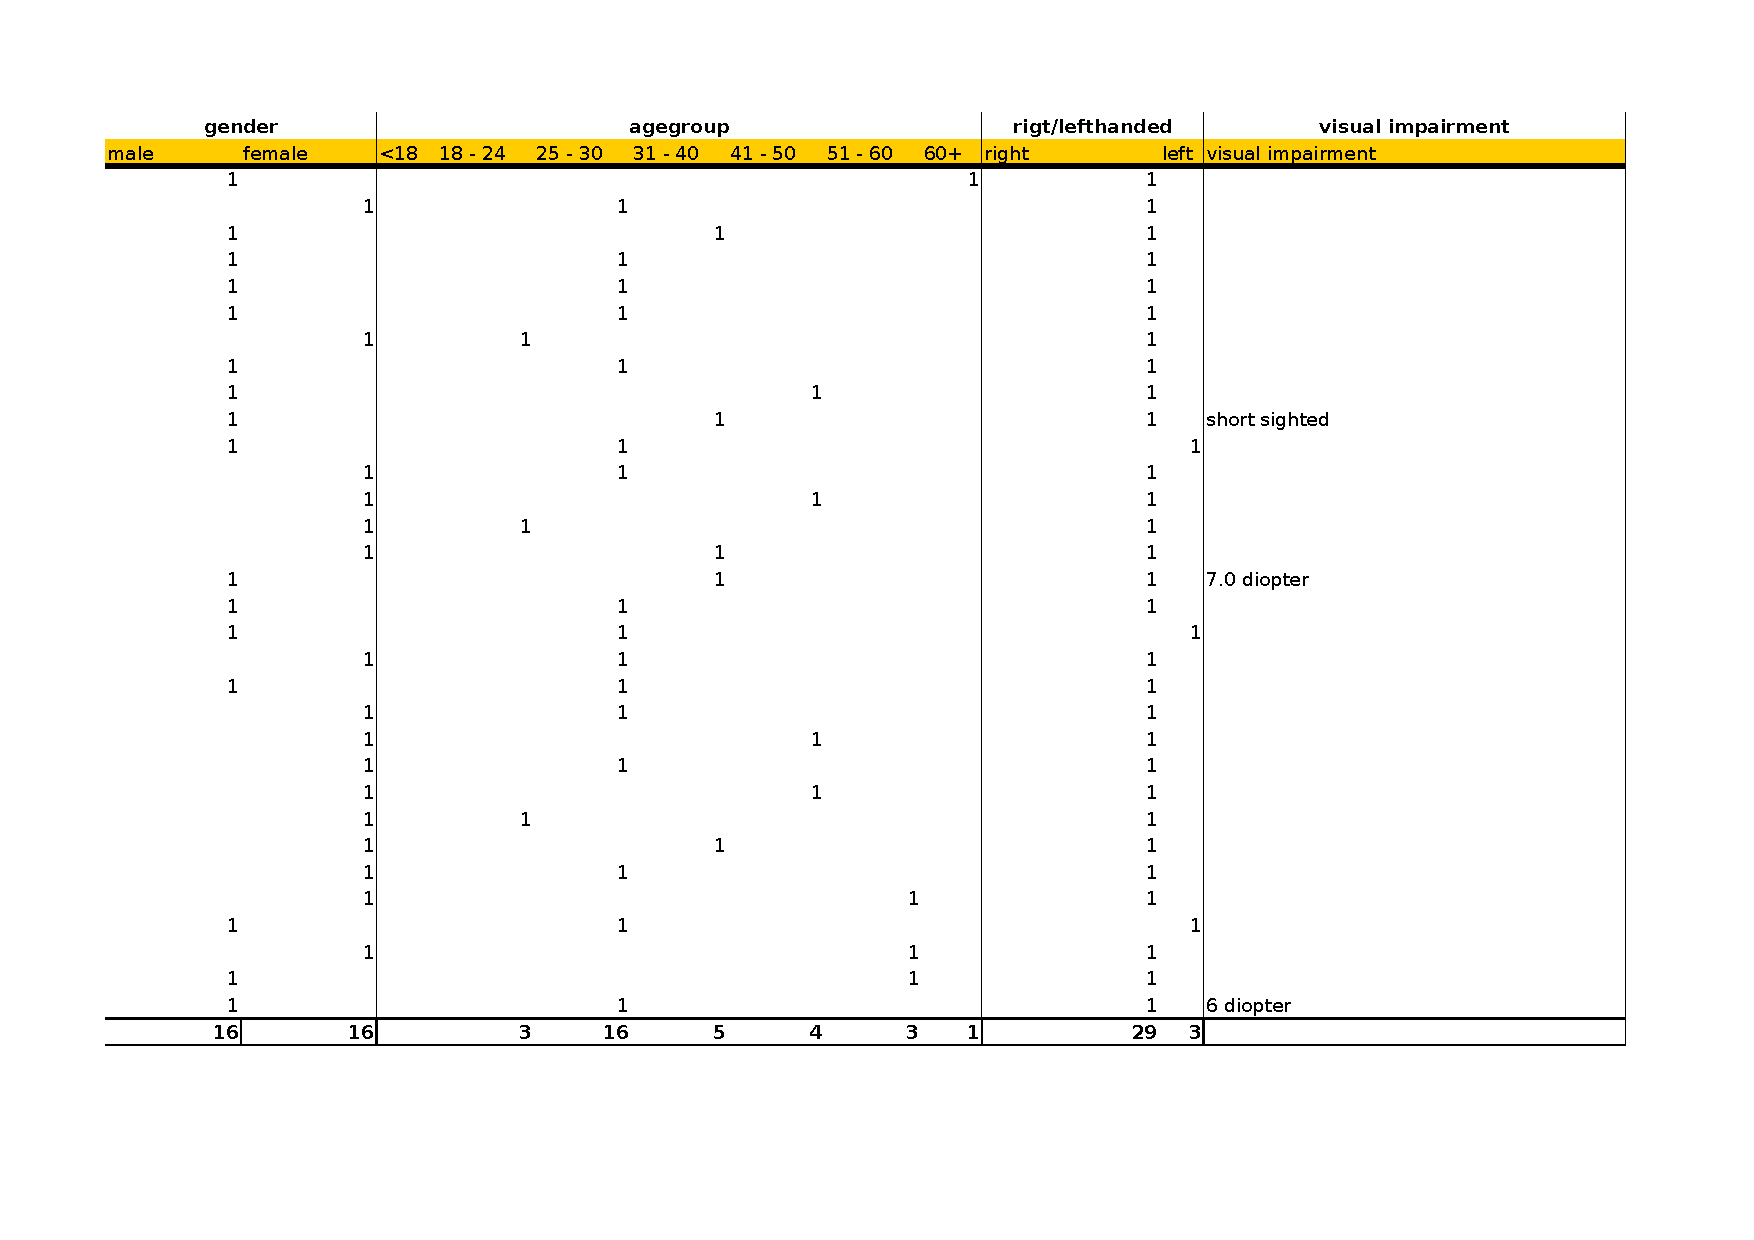
\includepdf[pages={1-2},angle=90]{appendix/userstudy_data_print.pdf}

\end{document}